%
% File emnlp2020.tex
%
%% Based on the style files for ACL 2020, which were
%% Based on the style files for ACL 2018, NAACL 2018/19, which were
%% Based on the style files for ACL-2015, with some improvements
%%  taken from the NAACL-2016 style
%% Based on the style files for ACL-2014, which were, in turn,
%% based on ACL-2013, ACL-2012, ACL-2011, ACL-2010, ACL-IJCNLP-2009,
%% EACL-2009, IJCNLP-2008...
%% Based on the style files for EACL 2006 by 
%%e.agirre@ehu.es or Sergi.Balari@uab.es
%% and that of ACL 08 by Joakim Nivre and Noah Smith

\documentclass[11pt,a4paper]{article}
\usepackage[hyperref]{emnlp2020}
\usepackage{times}
\usepackage{latexsym}
\renewcommand{\UrlFont}{\ttfamily\small}
\usepackage{todonotes}
\usepackage{enumitem}
\usepackage{amssymb}
\usepackage{tabularx}
\usepackage{subcaption}
\usepackage{booktabs}
\usepackage{multirow}
\renewcommand{\arraystretch}{1.2}

% This is not strictly necessary, and may be commented out,
% but it will improve the layout of the manuscript,
% and will typically save some space.
\usepackage{microtype}

%\aclfinalcopy % Uncomment this line for the final submission
%\def\aclpaperid{***} %  Enter the acl Paper ID here

%\setlength\titlebox{5cm}
% You can expand the titlebox if you need extra space
% to show all the authors. Please do not make the titlebox
% smaller than 5cm (the original size); we will check this
% in the camera-ready version and ask you to change it back.

\newcommand\BibTeX{B\textsc{ib}\TeX}

\title{Spot The Bot: A Robust and Efficient Framework for the Evaluation of Conversational Dialogue System}

\author{First Author \\
  Affiliation / Address line 1 \\
  Affiliation / Address line 2 \\
  Affiliation / Address line 3 \\
  \texttt{email@domain} \\\And
  Second Author \\
  Affiliation / Address line 1 \\
  Affiliation / Address line 2 \\
  Affiliation / Address line 3 \\
  \texttt{email@domain} \\}

\date{}

\begin{document}
\maketitle
\begin{abstract}
We introduce \emph{Spot The Bot}, a framework for evaluating conversational dialogue systems (chat bots) that aims at addressing several shortcomings in current evaluation approaches. In its core, \emph{Spot The Bot} relies on conversations between the bots that are to be evaluated, alleviating the need to create human-bot conversations which are time- and cost-intensive to create. 
These conversations are then, mixed with conversations between humans, shown to human annotators who decide which of the participants are bots. In the evaluation of these annotations, bots are ranked regarding their ability to disguise as humans. We empirically show that \emph{Spot The bot} is a robust and time-efficient method for evaluating chat bots by applying it to three domains, evaluating several state-of-the-art chat bots and drawing comparison to related work. The framework is released as a ready-to-use tool.
\end{abstract}

\section{Introduction}\label{sec:intro}
\noindent{\bf Motivation} Evaluation is a long-standing issue in the development of conversational dialogue systems (i.e.\ chat bots). The underlying difficulty in evaluation lies in the nature of the problem: Chat bots do not solve a clearly-defined task whose success is measurable in relation to an a priori defined ground truth. A common practice thus has become to aggregate subjective human judgements on a bot's success regarding criteria which often do not share a common, standardized definition. Such approaches entail further issues regarding evaluation: Gathering these human judgements is time- and cost-intensive, in addition to often yielding low agreement. The required cost- and time efforts also inhibit the repetition of such evaluations which raises questions on the robustness and thus significance of the results. 
Furthermore, current evaluations are based on single-turn ratings, which disregards the multi-turn nature of a dialogue. Although more and more multi-turn evaluations are performed, most of them are based on human-bot conversations, which are costly to obtain and suffer from low quality. \\
\noindent{\bf Contributions.}  In this work, we present the \emph{Spot The Bot} framework, an efficient evaluation methodology, which can be used to reliably discriminate different dialogue strategies. \emph{Spot The Bot} is based on the observation that conversational dialogue systems are trained on conversations between humans, and thus, the dialogue systems should be evaluated regarding their ability to mimic human behavior. \emph{Spot The Bot} works by  generating conversations between bots and letting crowd workers decide for each entity in the conversation if it is a human or a bot. It further allows to pin down features that contribute to a dialogue system's performance, enabling interpretable results (see Figure \ref{fig:motiv} for an overview). \\
 We show that our framework produces reliable, repeatable results, while being quicker and more cost-effective to run than related approaches, as it does not rely on human-bot conversations and generally requires fewer annotations. Furthermore, we show that disagreement between human annotators can be interpreted as a feature of a system's performance, rather than as a weakness in the evaluation approach. We apply the framework to three well-known domains as well as common baselines to produce a stable ranking among them. We release the framework as a ready-to-use tool for evaluating dialogue systems into which different systems can be plugged and compared\footnote{URL PLACEHOLDER}.

\begin{figure*}
    \centering
    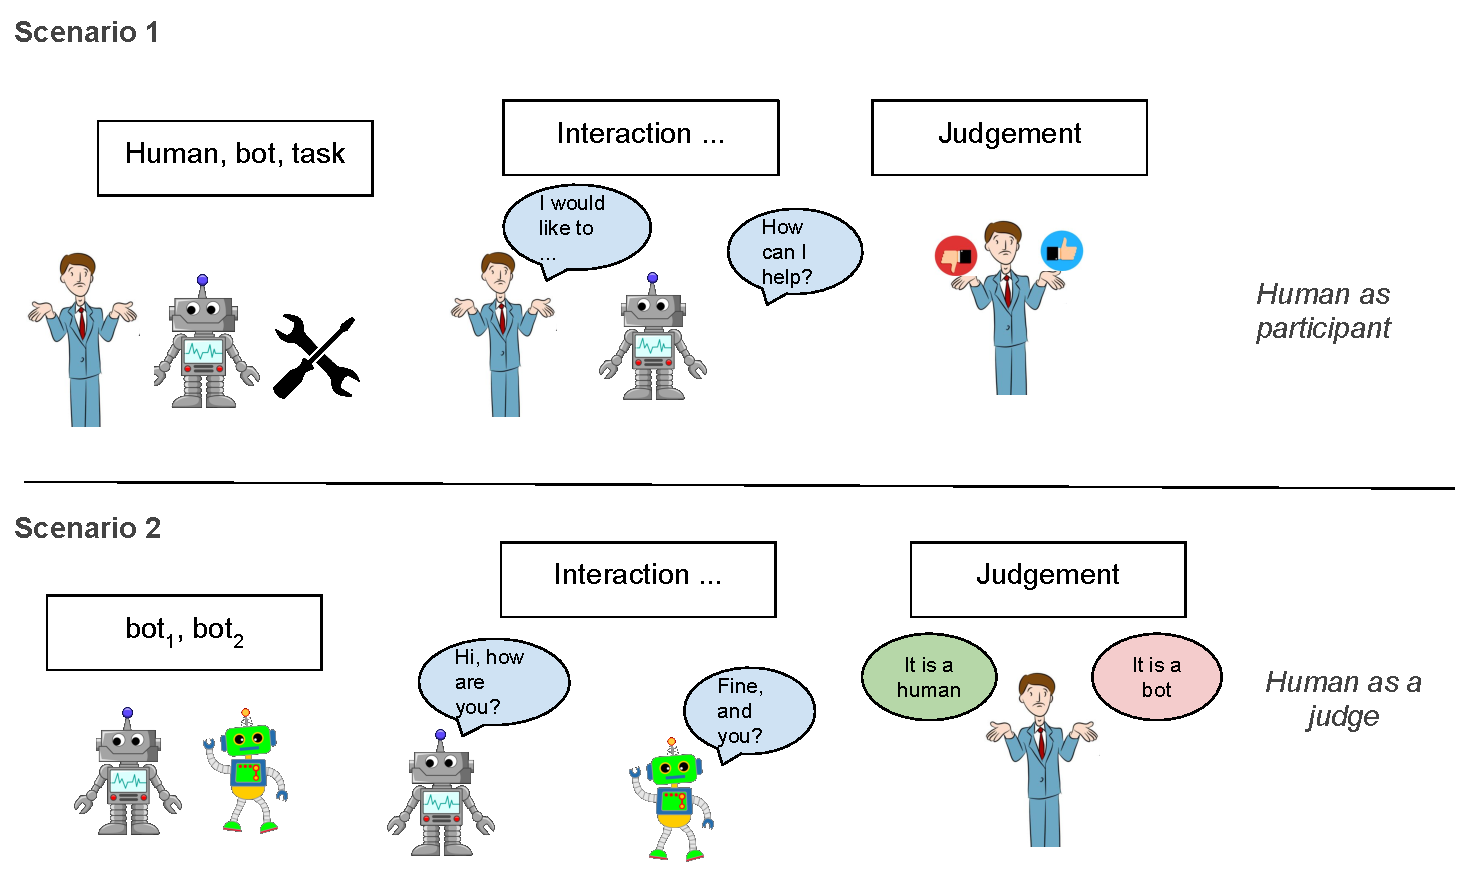
\includegraphics[scale=0.5]{figures/motivation_example_spotTheBot.pdf}
    \caption{Description of the main differences between the dialog systems evaluation methodology, in state of the art (scenario 1) and our model Spot The Bot (scenario 2).}
    \label{fig:motiv}
\end{figure*}

\section{Related Work}
\label{sota}

Nowadays there exist many methods to evaluate dialogue systems, both automatic and human-based, but unfortunately there is no single evaluation metric that is widely agreed upon in the scientific community \cite{deriu2019survey}. Task oriented dialogues can be evaluated based on whether the task is successfully accomplished, but open domain chit-chat systems, which do not have a precise goal, are more challenging to evaluate. Automatic evaluation metrics on chit-chat systems are problematic and are known to correlate poorly with human ratings~\cite{liu-etal-2016-evaluate,lowe-etal-2017-towards}. \\
\noindent{\bf Likert scale.} Most human evaluation are performed based on a Likert scale. However, Likert scores are known to suffer from high annotation variance,  are prone to order effects, are less reliable than participant ratings and have received much criticism~\cite{amidei-etal-2019-use}. In any case, human based evaluation is expensive and time consuming, and results are difficult to compare across different studies \cite{van-der-lee-etal-2019-best,amidei2019agreement}. \\
\noindent{\bf Single-turn evaluations.} Evaluations based on a static context and a single response from the dialogue systems are widely adopted, as they are time and cost efficient. Automated metrics that correlate with human scores exits in this setting~\cite{lowe-etal-2017-towards,mehri2020usr}. However, single-turn evaluation fails to capture the quality of the conversation as a whole.  For instance, a system that tends to produce repeated answers cat obtain a high single-turn score, albeit a low multi-turn one. \\
\noindent{\bf Human-Bot conversations.}  In order to perform multi-turn evaluations, the standard method is to let humans converse with the dialogue system and rate it afterwards. For instance, the ConvAI2 challenge~\cite{convai12} as well as the Alexa Prize~\cite{venkatesh2018evaluating} applied this procedure. There are several issues with this approach. First, it puts a high cognitive strain on the humans, as they have to perform several tasks at once~\cite{SCHMITT201512}. Second, it is hard to get high quality conversations. In fact, in the ConvAI2 challenge half of the collected human-bot conversations were discarded due to their low quality~\cite{convai12}. \\
\noindent{\bf Self-talk.} Recently, the idea of using self-talk dialogues, that is, dialogues where the bot talks to itself gained traction as a more cost efficient basis for evaluation~\cite{ghandeharioun2019approximating,li2019acuteeval,deriu-cieliebak-2019-towards}. For instance, in ACUTEval~\cite{li2019acuteeval} the authors evaluate bots that are self-chatting, and show that the results are comparable to human-bot chats. However, the humans need to read two dialogues by two different bots and decide which bot performed better with respect to various features. This increases the cognitive strain on annotators, as well as not being the optimal basis for direct comparisons between two bots. \\
\nodindent{\bf Turing Test.} \emph{Spot The Bot} is reminiscent of the Turing test, as the dialogue systems are evaluated based on their ability to mimic human behaviour. The Turing test has been criticized as a way to identify intelligence in NLP systems. For instance, \citet{bender-2020-acl} argue that a system may fool a user into believing it is human, and yet this does not prove that the system understands the meaning of the conversation they are having. However, in this paper we claim that \emph{failing} the test is a valid indicator that helps discriminate among bots that are competing with each other. Besides, we presume that eventually all the bots will fail the test, and hence we also collect a time component to record how much time it took for the bot to cheat the human.




\section{Spot The Bot}

In this section, we first provide an overview of the \emph{Spot The Bot} framework and then describe the individual steps of the evaluation process.

%\subsection{Motivation}
%In most of the evaluation methods described in section \ref{sota}, the evaluation of a dialogue system is based on human interactions and time consuming. Most of those methods can be described as in the scenario 1 of figure \ref{fig:motiv}, where given a specific task, a human interacts with the system and then decide if the system helped solving the task. This method focuses at the interaction and answers quality of one system at a time. Rather than evaluating the bot answers by a human, we consider an interaction between at least two different systems, then assess the quality of each system's answers. This process is highlighted in the scenario 2 of figure \ref{fig:motiv}, where, independently from a task, a human is a judge that decide if a given system is good or not, based on its answer. Such that, we consider a system as good, if the judge consider it as a human.

\subsection{Overview}
\label{sec:setting}
% figure
%----------------------------------------------------------------------------
\begin{figure*}
    \centering
    %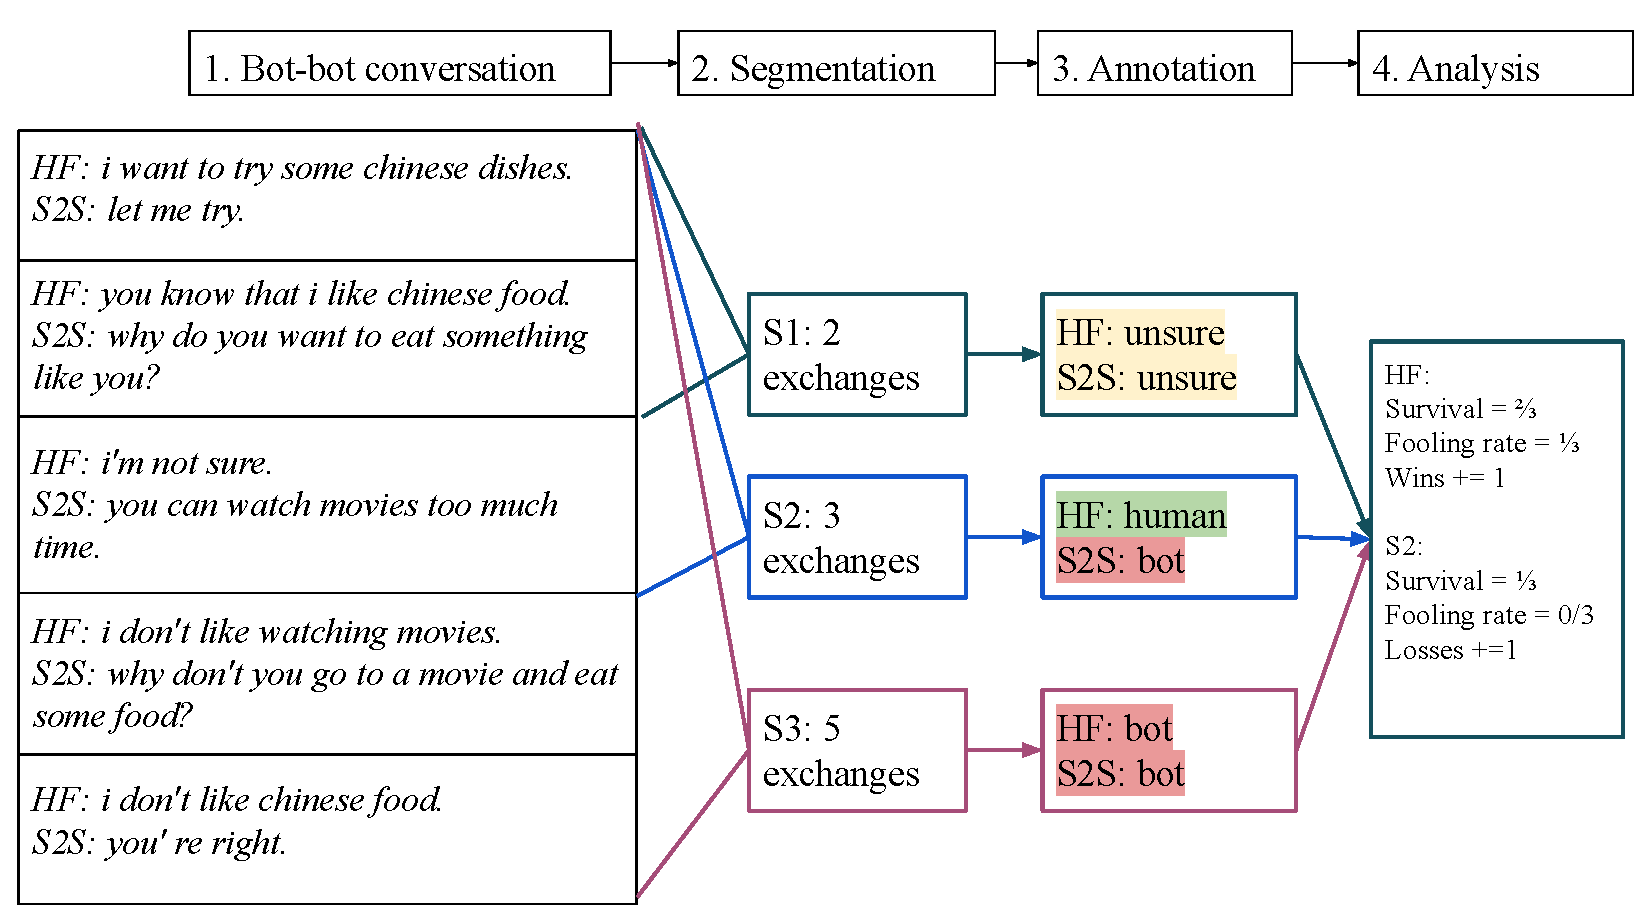
\includegraphics[scale=0.5]{figures/Copy of Spot the bot - annotation example - sketch2.pdf}
     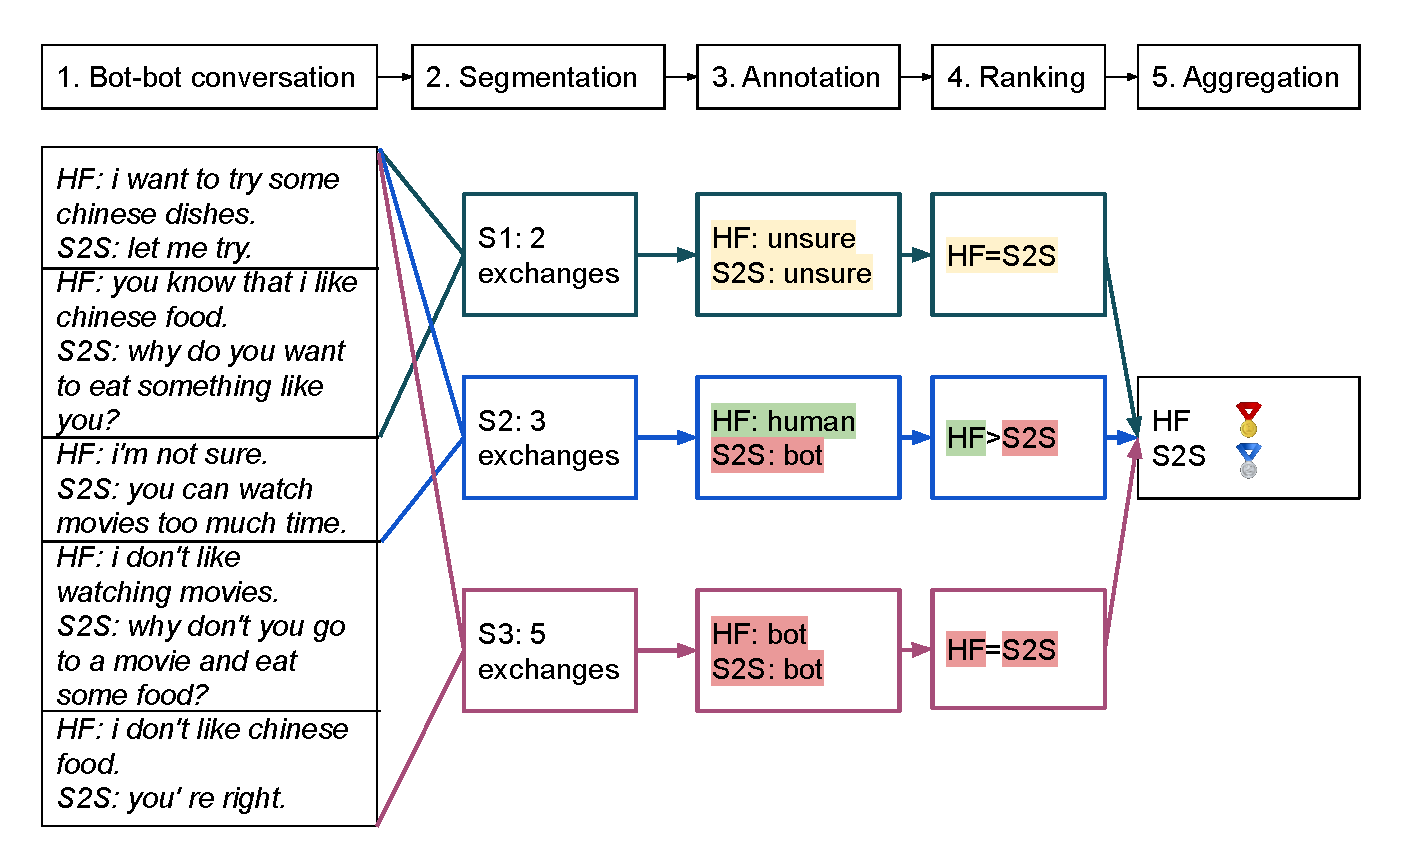
\includegraphics[scale=0.5]{figures/Spot the bot - annotation example - sketch2.pdf}
    \caption{Overview of the Spot The Bot process for one conversation. 1: A bot-bot conversation is segmented into different lengths (2, 3, and 5 exchanges). 2: These are show to distinct sets of annotators who judge whether each entity is a bot. 4: The winner is determined for each annotated segment and survival statistics are updated. This process is repeated for all conversations between the competing bots.}
    \label{fig:example}
\end{figure*}
%----------------------------------------------------------------------------
\emph{Spot The Bot} employs a tournament among conversational dialogue systems (bots) to determine which performs the best at mimicking the conversational behavior of humans. To measure the success of each bot, human crowd workers are shown conversations between the competing bots, mixed with conversations between humans. The crowd workers' task is then to determine for each participant in a conversation whether it is a human or a bot (or whether they are unsure). The bot that is most frequently annotated as being human, wins the tournament. Figure \ref{fig:example} provides an overview of the process for one conversation. \\
More formally, assume that there is a pool of $B$ bots $\{B_1, ..., B_B\}$, which is to be ranked, e.g.\ when a novel dialogue strategy is to be compared against existing strategies. For each pair of bots, a set of conversations is sampled by letting the bots talk to each other, where $S_{ij}$ denotes the set of conversations between $B_i$ and $B_j$. Each conversation is defined as a sequence of exchanges $e_0, ..., e_N$, where each exchange consists of two turns: $e_i = \{t_0^{e_i}, t_1^{e_i}\}$, one for each entity. % These conversations are sampled by priming the bots on contexts from the test set. Note that these contexts are not shown to the annotators, as they are not part of the bots’ output.\\
\noindent{\bf Segmentation.} The more exchanges there are in a conversation, the more likely it is that a bot gets recognized as such. Thus, we show different segments to the crowd workers. That is, we show the conversation at different stages $S_{ij}^k = e_0, ..., e_k$, where we chose different sets of values for $k$ depending on the domain \footnote{We experimented with letting crowdworkers decide themselves when to decide the exchange at which they were sure that an entity in the conversation is a bot or a human. However, this approach required too much fine-tuning to elicit the desired behaviour, cf.\ Appendix \ref{sec:appendix_gamification}.}.  Each segment of the same conversation is rated by a different annotator to avoid that one annotator sees the same conversation multiple  times, which would bias the rating. We choose multiple different segment lengths since we cannot know a priori which single length leads to a distinguishable difference between bots.\\
\noindent{\bf Human Conversations.} In order to establish an upper bound, we also add conversations among humans, which are sampled form the training material to be rated. These human conversations also serve as distractions to avoid that annotators start rating all the bots as humans due to potentially low quality of the bots.\footnote{We investigated whether the annotators realize that conversations are either between bots or humans by looking at ratios of conversations where both entities are labeled identically, but found no evidence that this happens more often than by chance.} \\
\noindent{\bf Annotation.} The annotation procedure works in two steps: First, the annotators have to decide for each entity in the conversation if it is a bot or a human. \\
Second, the framework allows to rate specific features, which are often used in current human evaluation (e.g. fluency, appropriateness, ...). The framework then measures the influence of these features on the survival time of the bots. There are two decisions to be made for the features: which features to rate (fluency, adequacy, quality, sensibleness, ... ) and how to rate them (Likert scale, continuous scale, pairwise comparison, ...).


\subsection{Ranking}
We define a win function for the annotations of the pairwise, direct conversations between the bots. The outputs of the win function are aggregated to determine the overall winner of the tournament. \\
\noindent{\bf Win Function.} Each annotations at each segment length $S_{ij}^k = e_0, ... , e_{k}$ constitutes the result of one annotation applied by one crowd worker, individually labeling each of the two conversation participants as either \textit{bot, human}, or \textit{unsure}. The winner of segment $S_{ij}^k$ under a crowd worker's annotation is determined by the following ordering of the labels: $\textit{human} >  \textit{unsure} > \textit{bot}$. That is, if bot $B_i$ is assigned the label \textit{human} and bot $B_j$ has label \textit{bot} or \textit{unsure}, $B_i$ has won the segment.\footnote{This process is repeated for all crowd workers who annotated the segment - in our case two per segment - and each win is counted separately.} Similar to \newcite{bojar-etal-2013-findings},  we define a win rate of $B_i$ against $B_j$ to aggregate the wins from all segments of all annotations stemming from conversations between bots $B_i$ and $B_j$, as: 

\begin{equation}\label{eq:win_function}
    %\textsc{win rate($B_i$, $B_j$)} =
    \frac{\textsc{wins($B_i, B_j$)}}{\textsc{wins($B_i, B_j$)} + \textsc{wins($B_j, B_i$)}}
\end{equation}
where $\textsc{wins($B_i$, $B_j$)}$ denotes the number of times that $B_i$ wins against $B_j$. \\
\noindent{\bf Ranking.} To create the ranking, we follow the approach by \newcite{dusek-etal-2018-findings} where the ranking is generated by the TrueSkill algorithm based on the win rate, and significant differences in performance are determined by bootstrap sampling. The result is a ranked set of clusters, where each cluster is composed of agents that do not have a significant difference in performance. 

\subsection{Survival Analysis}

We argue in Section \ref{sec:intro} that a bot that stays hidden longer is in a sense better. Therefore we apply survival analysis to assess the time it takes before a bot is spotted.

Survival analysis has a long history in the medical domain, where it is used, for example, to estimate the effect of different treatments on the long term survival rate of patients. In engineering disciplines it can be used for example to estimate the time to failure of certain machine components.

In our case, we are interested in the time, corresponding to the number of exchanges, until a dialogue system is spotted as such. We interpret the data gathered (see Section \ref{sec:setting}) as such: the ``spotted'' event occurred if the system was annotated as ``bot'' and it survived if it was annotated as ``unsure'' or ``human''. Let $N$ be the number of exchanges in the the annotated conversation segment, meaning that each dialog system produced $N$ outputs. If the dialog system was not spotted, then we know it survived for at least $N$ exchanges. For survival analysis this is a so-called right-censored data point. In case the dialogue system was spotted as such, we cannot tell the exact number of exchanges it took for an annotator to spot it, meaning it could have taken less than $N$ exchanges to spot. We therefore record that the spotting event happened in the interval $(0, N]$, a so-called interval-censored event.

From this data we can get non-parametric estimates of the survival function of the different systems per domain \citep{nonparametric_survival_censored}.  To check whether these differences are significant, we apply a generalized log-rank test \citep{generalized_logranktest_zhao2004}.

The field of survival analysis also offers different models for relating various covariates to the survival time. One of the most prominent among such models is the \emph{Cox Proportional Hazards Model} \citep{cox_ph_model}, which we use to study the influence of the different features outlined in Section \ref{sec:setting} on the time before the systems are spotted.\footnote{We use the \emph{icenReg} R package \citep{icenReg}, which allows us to fit a Cox model to our interval-censored data} This approach lets us compare bots in more detail and offers researchers insight into the reason of their bot's result in our evaluation.

Note that ranking based on win rates and survival analysis are complementary metrics. While the win rates-based ranking of the bots is a relative metric that is dependant on the pool of the selected bots, survival analysis is a metric whose output can be interpreted for each bot individually, independent of the other, competing bots. That is, the ranking based on win rates determines which bot performs best in a pool of bots, while survival analysis indicates how well a bot performs in absolute terms.

\section{Experiments}
We apply \emph{Spot The Bot} to three widely used domains for conversational dialogue systems: PersonaChat \cite{zhang-etal-2018-personalizing}, Dailydialog \cite{li-etal-2017-dailydialog}, and Empathetic Dialogues \cite{rashkin-etal-2019-towards}. For each domain, we prepared a pool of bots to be ranked and analysed. For each pair of bots, we sampled $|S_{ij}| = 45$ conversations. For the annotation task, we recruited paid crowdworkers from Amazon Mechanical Turk (AMT). In order to avoid that the results are biased towards the performance of a few crowdworkers, we designed a HIT as a batch of 20 conversations and each worker was only allowed to work on three batches. We designed the batches so that two segments of the same conversations never appear in the same batch, and each batch contains different segments of different conversations.  \\
\noindent{\bf Features.} We chose three features: sensibleness and specificity \cite{adiwardana2020towards}, which are shown to capture the core conversational behaviour of answering sensibly and not with illogical statements, while being specific to the given context of the conversation. The third feature is fluency, which states if the utterances are grammatically correct and fluent. The features are rated by preference ranking, that is, the annotator states which of the two entities performed better with respect to the features. This allows to compute the win-rates on the feature basis which makes comparisons between entities more stable \cite{yannakakis2011ranking}. \\
\noindent{\bf Segmentation.} The segment lengths are based on the lengths of the dialogues in a domain. PersonaChat and Dailydialog have longer conversations. Thus, we used segments of 2,3, and 5 exchanges. The Empathetic Dialogue domain has rather short dialogues, thus, we used segment lengths of 1,2, and 3 exchanges. We noted that having too long conversations leads to more cognitive strain on the annotators. 

\subsection{Dialogue Systems}
For the PersonaChat domain, we prepared a pool of $|B| = 6$ different dialogue systems: The Blender\footnote{Due to GPU restrictions, we used the small model with 90M parameters.} system (BL) \cite{roller2020recipes}, which is a state-of-the-art dialogue system trained on different domains, Lost in Conversation\footnote{\url{https://github.com/atselousov/transformer\_chatbot}} (LC) and Huggingface~\footnote{\url{https://github.com/huggingface/transfer-learning-conv-ai}}(HF), which were the top rated dialogue systems in the ConvAI2 challenge \cite{dinan2020convai2}, KVMemNN (KM), which is the baseline used for the ConvAI2 challenge, and two systems trained with ParlAI \cite{miller2017parlai}: BertRank (BR), and a small Seq2Seq model (DR). The small Seq2Seq model is trained only for 3 epochs, and returns only very general and short answers, which serves to assess how Spot The Bot works for very weak models.  \\
For the Empathetic Dialogues domain, we used a set of $|B| = 5$ dialogue systems using the ParlAI framework: The Blender model (BL), a fine-tuned GPT2 (GPT), BertRank (BR), Seq2Seq+Att (S2), and a small Seq2Seq model (DR).  \\
For the Dailydialog domain, we used the same set of systems as the Empathetic Dialogues, except for the Blender model.



\subsection{Ranking Results}
\begin{table}[h!]
\centering
\small
\scalebox{0.75}{
\begin{tabular}{l|cccccc|cc} 
\multicolumn{9}{c}{Dailydialog} \\
\toprule
\textsc{} & \textsc{GPT} &  \textsc{BR} &  \textsc{S2} & \textsc{DR} & & & \textsc{Win Rate}& \textsc{Range}\\
\hline 
\textsc{GPT} & -             & \textbf{0.67} & \textbf{0.77} & \textbf{0.93} & & & 0.79 & (1,1) \\
\textsc{BR} & \textbf{0.33} & -          & \textbf{0.79}    & \textbf{0.83} & & & 0.65 & (1,2)  \\
\textsc{S2} & \textbf{0.23} & \textbf{0.21} & -             & \textbf{0.74} & & & 0.39 & (3,3) \\
\textsc{DR} & \textbf{0.07} & \textbf{0.17} & \textbf{0.26} & -             & & & 0.16 & (4,4) \\
\bottomrule
\multicolumn{9}{c}{Empathetic Dialogues} \\
\toprule
\textsc{} & \textsc{BL}& \textsc{BR} &  \textsc{GPT} &  \textsc{S2} & \textsc{DR} & & \textsc{Win Rate} & \textsc{Range}\\
\hline 
\textsc{BL}& - & \textbf{0.82} & \textbf{0.83} & \textbf{0.9} & \textbf{0.94} && 0.87 & (1,1)  \\
\textsc{BR}& \textbf{0.18} & - & 0.51 & \textbf{0.77} & \textbf{0.93} && 0.59 & (2,3)  \\
\textsc{GPT}& \textbf{0.17} & 0.49 & - & \textbf{0.61} & \textbf{0.73} && 0.50 & (2,3) \\
\textsc{S2}& \textbf{0.10} & \textbf{0.23} & \textbf{0.39} & - & \textbf{0.63} && 0.33 & (4,4) \\
\textsc{DR}& \textbf{0.06} & \textbf{0.07} & \textbf{0.27} & \textbf{0.37} & - && 0.19  & (5,5)\\
\bottomrule



\multicolumn{9}{c}{PersonaChat} \\
\toprule
\textsc{} & \textsc{BL}& \textsc{LC} &  \textsc{KV} &  \textsc{HF} & \textsc{BR}  & \textsc{DR} &\textsc{Win Rate} & \textsc{Range}\\
\hline 
\textsc{BL}& - & 0.56 & \textbf{0.68} & \textbf{0.72} & \textbf{0.84} & \textbf{0.95}&  0.75 & (1-1) \\
\textsc{LC}& 0.44 & - & 0.54 & \textbf{0.72} & \textbf{0.75} & \textbf{0.89} & 0.69  & (2-3)\\
\textsc{KV}& \textbf{0.32} & 0.46 & - & \textbf{0.77} & \textbf{0.74} & \textbf{0.91} & 0.64 & (2-3)\\
\textsc{HF}& \textbf{0.28} & \textbf{0.28} & \textbf{0.23} & - & \textbf{0.63}& \textbf{0.89} & 0.46& (4-4)\\
\textsc{BR}& \textbf{0.16} & \textbf{0.25} & \textbf{0.26} & \textbf{0.37} & - & \textbf{0.75} & 0.35& (5-5) \\
\textsc{DR}& \textbf{0.05} & \textbf{0.11} & \textbf{0.09} & \textbf{0.11}& \textbf{0.25} & - & 0.12& (6-6) \\
\bottomrule
\end{tabular}
}
\caption{Win rates for each pair of systems for each of the three domains. The bold entries denote significance ($p < 0.05$) computed with Chi-square test. The ranking ranges are computed using bootstrap sampling. The rank ranges are the ranges in which the bot falls in at least 95\% of cases. Two bots are distinct if there is no overlap in the ranges of their respective cluster.}
\label{tab:win_rates}
\end{table}
Table \ref{tab:win_rates} gives an overview of the win rates for each pair of dialogue systems as well as the ranking ranges, which denote the clusters. The significance is computed by the Chi-square test. For each domain, most pairwise win-rates are significant. \\
As expected DR performs worst in all three domains, which is due to its repetitive nature, which is exposed over the course of a dialogue. In the Dailydialog domain and the Empathetic Dialogues domain, the GPT2 and the BR models perform equally, i.e. they end up in the same cluster. In both domains, the language models outperform the S2 model, which is in line with the expectation of large and powerful language models outperforming previous state-of-the-art models.
The BL model outperforms all other models in both the PersonaChat and Empathetic Dialogues domains, which is in line with the results presented by the authors of the Blender model. The pairwise comparison of BL to the LC model is not significant in our case, which is probably due to the fact that we used the small version of the BL model. Furthermore, the LC model is ranked very highly. This corresponds to the findings of the ConvAI2 challenge. However, in Spot The Bot, the KV is ranked much higher than the Huggingface model, which is not in line with the ConvAI2 evaluation. 


\subsection{Survival Analysis}

% figure
%----------------------------------------------------------------------------
\begin{figure*}[h!]
  \begin{subfigure}[b]{0.3\textwidth}
    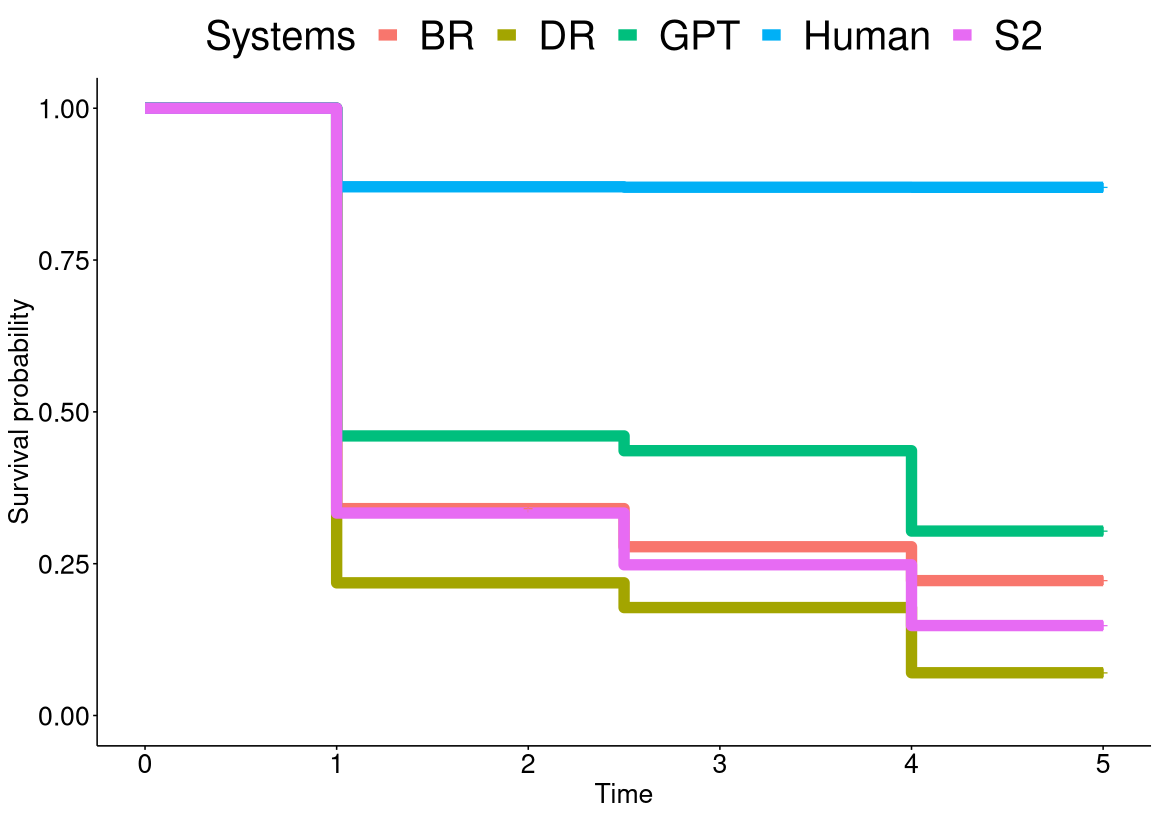
\includegraphics[width=\textwidth]{figures/survival/dailydialog_all.png}
    \caption{Dailydialog}
  \end{subfigure}
  \begin{subfigure}[b]{0.3\textwidth}
    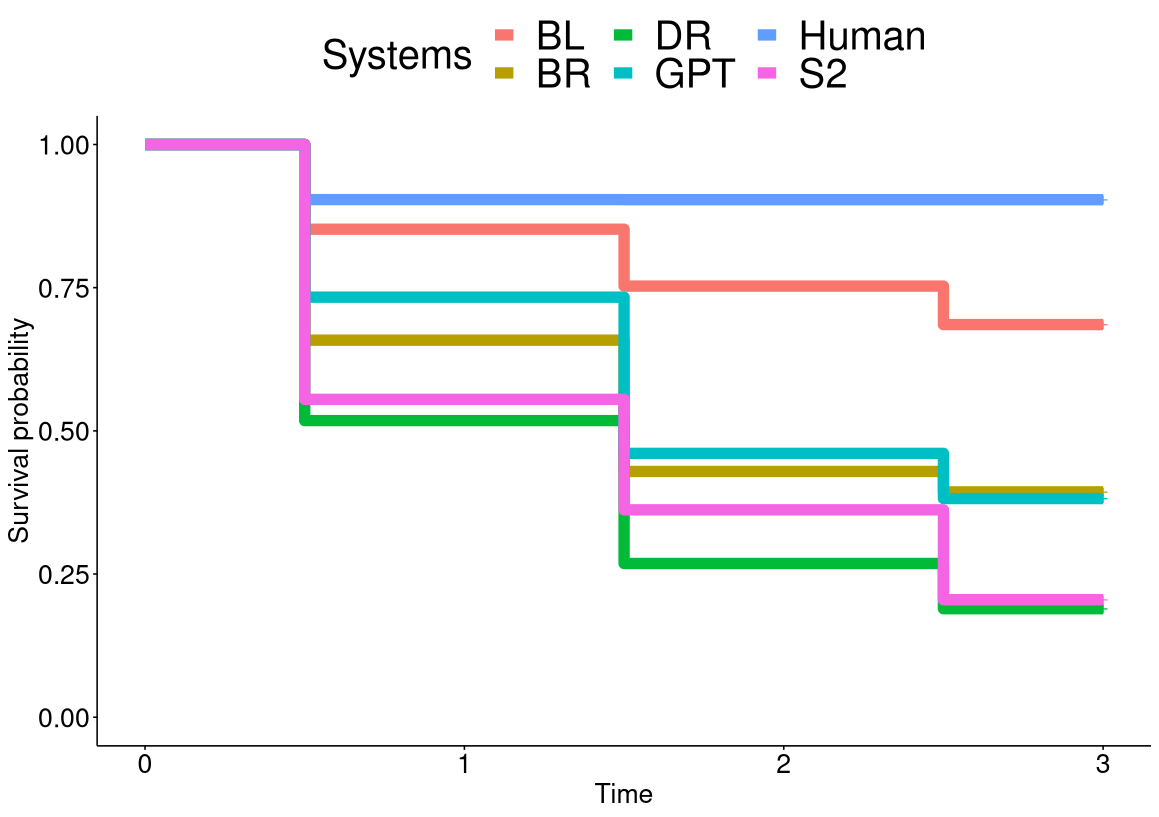
\includegraphics[width=\textwidth]{figures/survival/empathetic_all.png}
    \caption{Empathetic Dialogues}
  \end{subfigure}
  \begin{subfigure}[b]{0.3\textwidth}
    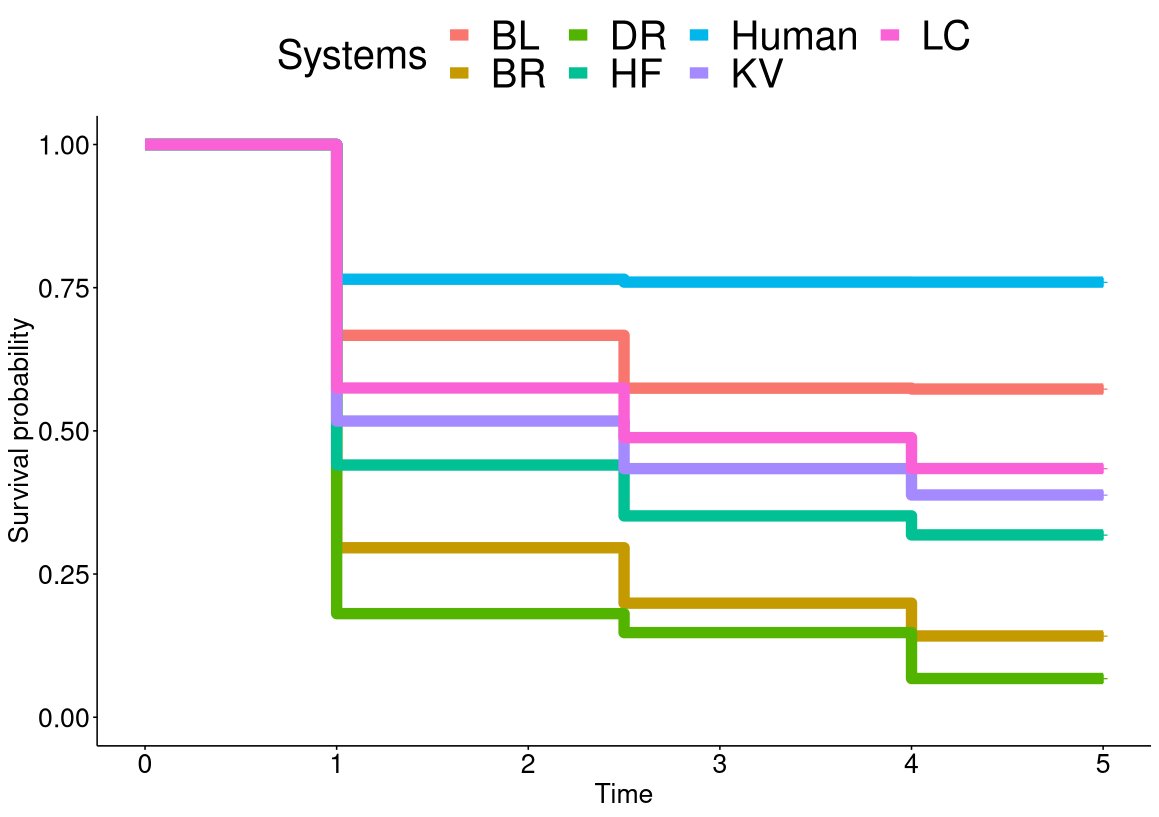
\includegraphics[width=\textwidth]{figures/survival/convai2_all.png}
    \caption{PersonaChat}
  \end{subfigure}
  \caption{Survival function per system estimated for each domain.}
  \label{fig:survival_all_domains}
\end{figure*}

Figure \ref{fig:survival_all_domains} shows the survival functions for the three domains. We see that there are differences in the survival of the different systems that correspond to the fooling rates observed in Figure \ref{fig:fooling_rate}. The survival rates imply the same rankings as those from pairwise win-rates reported in Table \ref{tab:win_rates}. The only exception being the Empathetic Dialogues domain, where GPT and BR switch places. Importantly, the distinction between these two is not significant in both rankings. Further non-significant differences are S2 and DR in the Empathetic Dialogues domain, BR and S2 in the Dailydialog domain, and LC and KV in the PersonaChat domain. All other pairwise comparisons of survival curves are significant with $p  < 0.05$ after correction for multiple comparisons.
\begin{table}[ht]
    \centering
    \small
    \begin{tabular}{l|ccc}
    
    \multicolumn{4}{c}{Dailydialog} \\
    \toprule
    & Fluency & Specificity & Sensibleness \\ \hline
    GPT & \bf 0.69 & 0.55     & \bf 0.77\\
    BR  & 0.77     & \bf 0.78 & \bf 0.62\\
    S2  & 0.31     & 0.52     & \bf 0.41\\
    DR  & \bf 0.23 & 0.15     & \bf 0.20\\
    \bottomrule
    
    %\vspace{0.5em}\\

    \multicolumn{4}{c}{Empathetic Dialogues} \\
    \toprule
    & Fluency & Specificity & Sensibleness \\ \hline 
    BL  & 0.84     & 0.79 & \bf 0.84\\
    GPT & \bf 0.51 & 0.42 & \bf 0.49\\
    BR  & \bf 0.60 & 0.65 & \bf 0.56\\
    S2  & \bf 0.33 & 0.47 & \bf 0.39\\
    DR  & \bf 0.21 & 0.17 & \bf 0.21\\
    \bottomrule
    
    %\vspace{0.5em}\\

    \multicolumn{4}{c}{PersonaChat} \\
    \toprule
    & Fluency & Specificity & Sensibleness \\ \hline
    BL  & \bf 0.73 & 0.74     & \bf 0.73\\
    LC  & 0.56     & 0.54     & \bf 0.62\\
    KV  & \bf 0.61 & 0.63     & \bf 0.58\\
    HF  & \bf 0.46 & \bf 0.46 & \bf 0.47\\    
    BR  & 0.48     & 0.44     & \bf 0.43\\
    DR  & \bf 0.16 & 0.19     & \bf 0.16\\
    \bottomrule

\end{tabular}
    \caption{Per feature win-rate of the different systems over all domains. Bold numbers indicate that the feature has a significant
    influence on system survival according to a Cox model.}
    \label{tab:survival_features}
\end{table}
\\
\noindent{\bf Feature Influence} For each of the three features -- fluency, specificity, and sensibleness -- annotators have to specify whether one entity performed better, the same, or worse than the other. We encode this information as $1$, $0$, and $-1$ respectively and fit a Cox proportional hazards model for every system independently with the features as covariates.

The numerical entries in Table \ref{tab:survival_features} refer to the per-feature win-rate of each bot, which is computed analogously to Equation \ref{eq:win_function} using the feature annotations directly. Using these can be more intuitive than relying on the magnitude of the model coefficients, which can be hard to interpret.
Bold entries in Table \ref{tab:survival_features} show which features have a significant influence on the system being spotted. All significant effects go in the intuitive direction, meaning that a higher feature value leads to longer survival.  For example, for the DR model, the fluency feature is significant across all three domains, and together with its low fluency win-rate, we can deduce that it is often spotted due to its low fluency. Sensibleness seems to be an important feature across the board, meaning that in general, bots can be spotted due to inappropriate, nonsensical answers or hide if they respond in a suitable manner. Interestingly, specificity seems to be mostly unimportant which could be due to either the bots not being noticeably unspecific, or it being an irrelevant feature for the chosen domains.

\section{Discussion}

\subsection{On Reliability}
One key requirement to an evaluation procedure is that repeated executions of the procedure result in the same outcome. We measure how many pairwise conversations between two bots are needed to guarantee a stable ranking. That is, what is the lower bound to $|S_{ij}|$ so that the ranking is stable. For each $|S_{ij}| \in \{3 ... 44\}$, we randomly sample $|S_{ij}|$ conversation for each pair and compute the ranking. We repeat this subsampling procedure a 1000 times, and measure the minimum $|S_{ij}|$ that guarantees the same ranking in at least $95\%$ of cases.
% figure
%----------------------------------------------------------------------------
\begin{figure}[h!]
  \begin{subfigure}[b]{0.45\textwidth}
    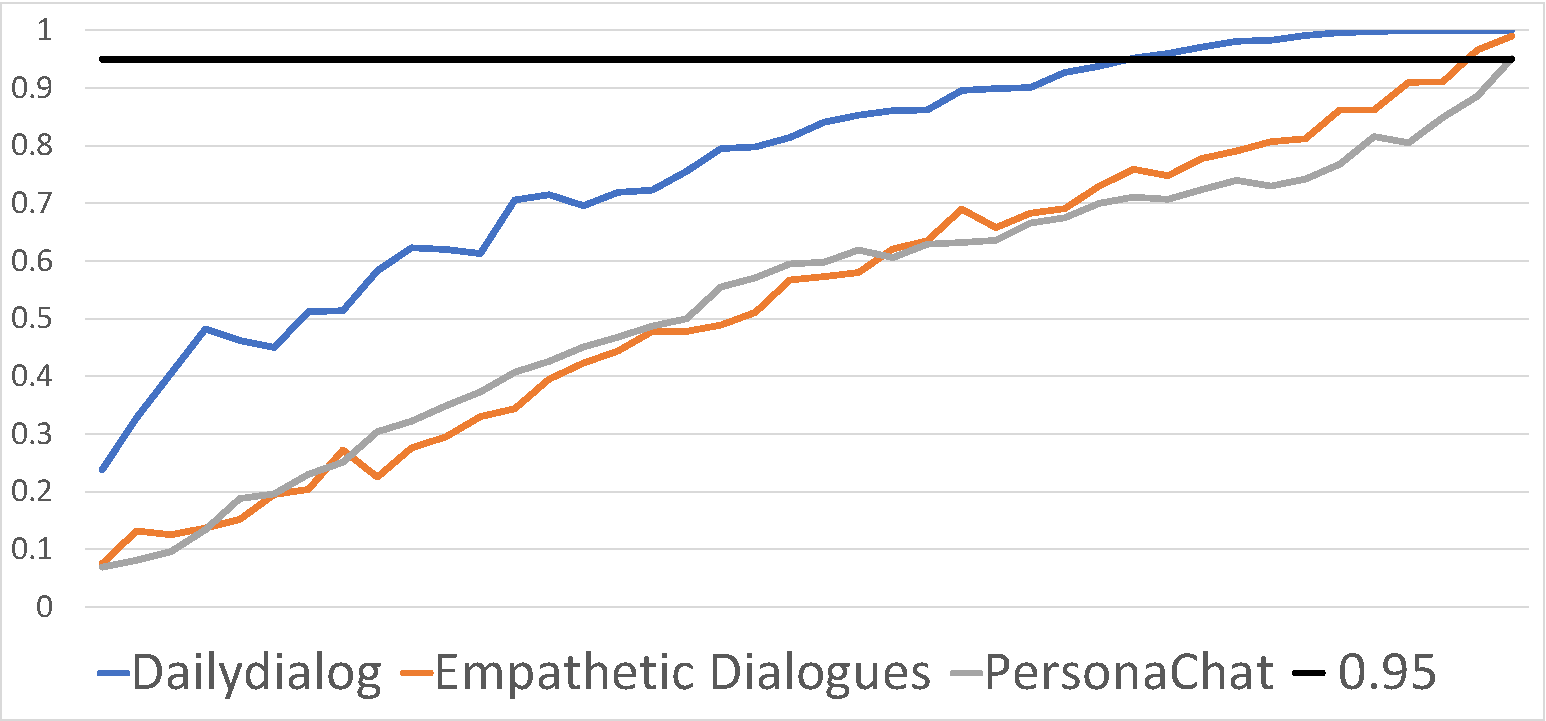
\includegraphics[width=\textwidth]{figures/rankig-sigificance.pdf}
    \caption{Stability Experiment.}
    \label{fig:ranking-significance}
  \end{subfigure}
  \begin{subfigure}[b]{0.45\textwidth}
    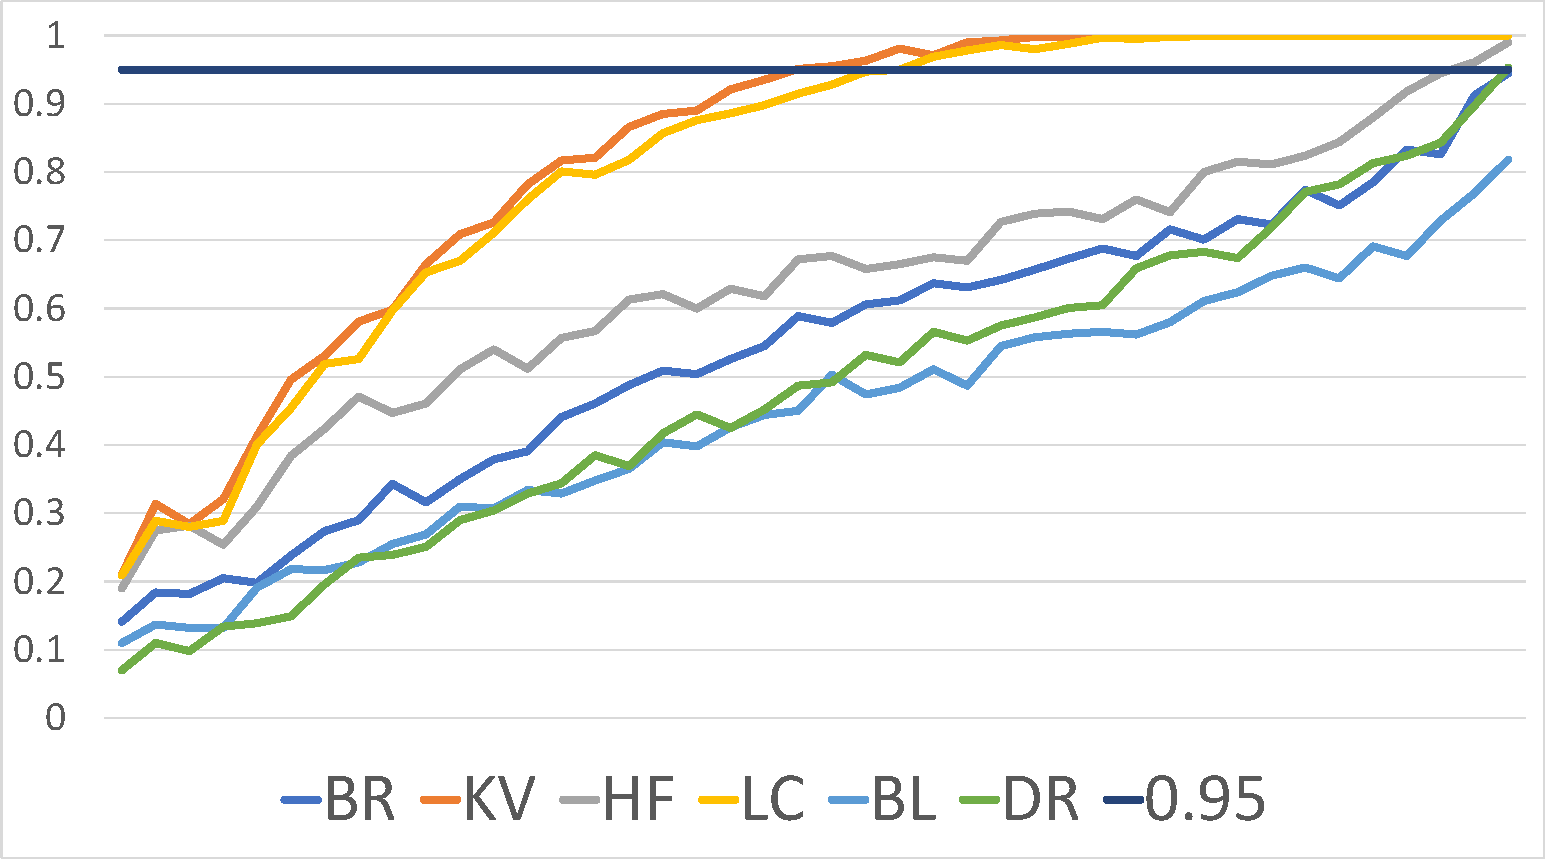
\includegraphics[width=\textwidth]{figures/rankig-sigificance-loo.pdf}
    \caption{Leave-one-out Experiment.}
    \label{fig:ranking-significance-loo}
  \end{subfigure}
  \caption{Ranking stability experiments.The x-axis denotes the number of pairwise conversations between two bots. The y-axis denotes the rate at which the same ranking is achieved across 1000 repetitions. The horizontal line denotes the 95\% mark. In the lower Figure, we show the experiments for the PersonaChat domain, when leaving one system out.}
\end{figure}
%----------------------------------------------------------------------------
Figure \ref{fig:ranking-significance} shows for each $|S_{ij}| \in \{3 ... 44\}$ the proportion of times in which the most frequent ranking occurred. For the Dailydialog domain $|S_{ij}| = 33$ pairwise conversations are enough to guarantee a stable ranking. In the other two domains this value is reached with over 40 pairwise dialogues. This is due to the fact that in these two domains there are dialogue systems, which are not distinguishable in their performance. In order to investigate this phenomenon, we repeat the above experiment on the PersonaChat domain by leaving one system out. Figure \ref{fig:ranking-significance-loo} shows the result of the ranking stability for each left-out system. When leaving one between LC or KV out, the stability is achieved with 25 pairwise dialogues, which is due to the fact that their pairwise comparison is not significant. However, a subsample of their pairwise comparisons might yield significant differences, which leads to different clusters in the ranking. In fact, the two rankings differ in that the first puts KV and LC in the same cluster, and in the second, LC and KV are in separate clusters, with LC being on top.

Methods based on human-bot interactions required more conversations as for example in ConvAI2, where they evaluated 100 dialogues per system.  ACUTE-EVAL, which is more similar to our method, obtained a high agreement evaluating pairs with 20 conversations per system, but they did not report agreement for the ranking of a pool of systems.

\subsection{Annotator (Dis)agreement as a Feature}
The robustness of evaluation of conversational dialogue systems is often hampered by inter-annotator agreement (IAA) \cite{gandhe2016semi}. % IAA is generally measured using some agreement metric, and the soundness of the evaluation data is determined by segmenting the range of such metrics into (non-)acceptable subranges. 
On the one hand, measuring and reporting IAA is, unfortunately, not a standard practise in the evaluation of chat bots \cite{amidei2019agreement}. On the other hand, it has been shown that producing annotations with high IAA on open domain conversations is a challenging endeavour, as annotating features on e.g.\ likert scales is prone to be impeded by subjective interpretation and idiosyncratic annotator behaviour \cite{bishop2015use}.
%The main goal for a bot in our setting is to disguise as a human, and the bot which manages to do so the longest, wins. 

In our setting, annotator disagreement on a bot's human-like behaviour can be interpreted as a feature: A bot that manages to fool one of two annotators (maximal disagreement) into believing it is human can be said to have performed better than a bot that does not manage to fool any annotator (maximal agreement). Conversely, a bot that is spotted with high agreement has performed worse than a bot that is spotted with lower agreement.
% Based on this intuition, we apply two measures of inter-annotator agreement, i.e.\ a) direct agreement between the annotated labels (human, bot, undecided) per entity, and b) agreement on the outcome of the win function (as defined above).

%In a first step, we calculate label agreement by the fraction of segments where an entity was annotated with the same label by both annotators. Table \ref{tab:label_agreement_dailydialog} shows the label agreement for the Dailydialog domain per segment length and bot. Random chance agreement is 0.33, given three labels. We see that all agreements are higher than agreement by chance and that agreement increases with the increase of the segment length, indicating that segment length plays an important role in the annotation task regarding agreement. Furthermore, we see that the bots that perform the weakest regarding fooling rates and ranking ({S2} and {D}) reach high agreement, i.e.\ for system {D}, its agreement is almost on par with the one for human entities.

%\begin{table}[ht]
%    \centering
%    \begin{tabular}{l|ccc|c}
%    \toprule
% & 2 & 3 & 5 & {Overall}\\ \hline
%\it human & \it 0.80 & \it 0.74 & \it 0.82 & \it 0.78\\ \hline
%BR & 0.54 & 0.62 & 0.70 & 0.62\\
%HF & 0.44 & 0.53 & 0.56 & 0.51\\
%S2S & 0.56 & 0.66 & 0.72 & 0.64\\
%D & 0.69 & 0.73 & 0.87 & 0.76\\
%\bottomrule
%    \end{tabular}
%    \caption{Label agreement per segment length in the Dailydialog domain.}
%    \label{tab:label_agreement_dailydialog}
%\end{table}

%This analysis tells us how well annotators agree in general, but does not indicate whether they agree on the level of human-like behaviour of each bot. 
To investigate this, we calculate per bot and label the percentage of cases where both annotators annotate the label if one of them does. Given three labels (\emph{human, bot, unsure}), the chance for random agreement is 0.33. A bot's goal in this analysis is to reach high agreement on the \emph{human} label (since it has then tricked both annotators into believing it is human) and low agreement on the \emph{bot} label (it is better to be spotted as a bot by only one annotator). Results are shown in Table \ref{tab:agreement_per_label}.

\begin{table}[ht]
    \centering
    \small
    \begin{tabular}{l|ccc}
    
    \multicolumn{4}{c}{Dailydialog} \\
    \toprule
    label & bot $\downarrow$ & human $\uparrow$ & unsure\\ \hline
    \it human & \it 0.28 & \it 0.88 & \it 0.07\\ 
    GPT & 0.64 & 0.38 & 0.14\\
    BR & 0.75 & 0.33 & 0.15\\
    S2 & 0.77 & 0.30 & 0.12\\
    DR &  0.88 &  0.14 & 0.15\\
    \bottomrule
    
    %\vspace{0.5em}\\

    \multicolumn{4}{c}{Empathetic Dialogues} \\
    \toprule
    label & bot $\downarrow$ & human $\uparrow$ & unsure\\ \hline
    \it human & \it 0.28 & \it 0.88 & \it 0.23\\ 
    BL & 0.33 & 0.72 & 0.21\\
    GPT & 0.66 & 0.57 & 0.15\\
    BR & 0.64 & 0.57 & 0.25\\
    S2 & 0.74 & 0.50 & 0.19\\
    DR & 0.78 & 0.46 & 0.28\\
    \bottomrule
    
    %\vspace{0.5em}\\

    \multicolumn{4}{c}{PersonaChat} \\
    \toprule
    label & bot $\downarrow$ & human $\uparrow$ & unsure\\ \hline
    \it human & \it 0.42 & \it 0.75 & \it 0.09\\ 
    BL & 0.43 & 0.58 & 0.06\\
    LC & 0.60 & 0.52 & 0.10\\
    HF & 0.70 & 0.41 & 0.10\\    
    KV & 0.64 & 0.49 & 0.08\\
    BR & 0.82 & 0.27 & 0.06\\
    DR & 0.90 & 0.28 & 0.08\\
    \bottomrule

    \end{tabular}
    \caption{Label agreement. Bots are sorted according to their ranking in the tournament.}
    \label{tab:agreement_per_label}
\end{table}

We observe that the bots that rank high in the tournament outcome and the survival analysis (BL, HF, LC) obtain the highest agreement on the \emph{human} label and lowest agreement on the \emph{bot} label in all domains. For the BL system in the Empathetic Dialogues domain, the agreement values are highly distinct from the other competitors and close to the agreement that the human entities obtain. That is, in 72\% of the cases where one annotator labels the bot as being human, the other annotator agrees. Conversely, the annotators agree that BL is a bot in only 33\% of the cases where one annotator identifies it as a bot. That is, the agreement for the \emph{human} label is more than twice as high as agreement by chance, and agreement on the \emph{bot} label is as low as random agreement. On the other end, we see that the DR system consistently obtains highest agreement when being identified as a bot, and lowest when it is perceived as a human. 
%The Dailydialog domain seems to be the hardest in terms of convincing both annotators of human-like behaviour, i.e.\ the agreement on the \emph{human} label for the best performing bot (HF) is only slightly higher than random agreement. 
Our analysis of the agreement on the assigned labels suggests that the ranking in our Spot The Bot experiments do not result from random agreement between the annotators, i.e.\ the annotations of the best and worst performing systems show agreements distinctly higher than chance regarding the respective labels. This is different from previous evaluations, specially those based on Likert scores, where it is difficult to obtain a high IAA \cite{bishop2015use}. Moreover, we take advantage of disagreement as an informative measure. ACUTE-EVAL, which is more similar to our method, reported agreement rates between 70\% and 87\% with only two labels (bot A or bot B) using PersonaChat.

%We see that {HF} reaches the best agreement on the \emph{human} label and the lowest on the \emph{bot} label. That is, if one annotators annotates it as being human, the other annotator does so as well in 38\% of the cases, and in 64\% percent of the cases where one annotator spots {HF} as a bot, the other annotator agrees. Conversely, system {D} again has the highest agreement regarding the \emph{bot} label and the lowest on the \emph{human} label. Overall, there is little agreement on the unsure label, indicating that a decision can be taken for most segments.

%\begin{table*}[ht!]
%    \centering
%    \small
%    \begin{tabular}{l|cccccc}
%    \toprule
%Bot & bot-bot & bot-human & bot-unsure & human-human & human-unsure & %unsure-unsure\\ \hline
%\it human & \it 0.04 & \it 0.16 & \it 0.03 & \it 0.74 & \it 0.03 & \it 0.00\\ %\hline
%BR & 0.54 & 0.24 & 0.11 & 0.07 & 0.02 & 0.01\\
%HF & 0.39 & \bf 0.30 & 0.13 & \bf 0.11 & 0.06 & 0.01\\
%S2S & 0.59 & 0.21 & 0.13 & 0.05 & 0.01 & 0.01\\
%D & \bf 0.74 & 0.13 & 0.08 & 0.01 & 0.03 & 0.01\\
%\bottomrule
%    \end{tabular}
%    \caption{Distribution over annotated label pairs for the Dailydialog %domain. }
%    \label{tab:label_pair_percentage}
%\end{table*}

%We extend this analysis to the level of conflicting label pairs.\footnote{Since we always have two annotators per segment, we obtain pairs of labels.} A label pair is the combination of the labels assigned to an entity in a segment. We calculate the distribution over label pairs found in the annotation per entity, shown in Table \ref{tab:label_pair_percentage}. We are here particularly interested in conflicting labels (\emph{bot-human, bot-unsure, human-unsure}). Since \emph{human-unsure} is quite rare, we focus on the other two. The most erratic label pair in terms of disagreement is the \emph{bot-human} label, indicating a vastly different impression of the bots' behaviour in the eyes of the annotators. We see that it is almost twice as frequent as the \emph{bot-unsure} label. Overall however, this problematic label confusion occurs in at most 30\% of the cases (HF), leaving the other 70\% with less severe disagreement.



\subsection{On Time efficiency}
Evaluation methods, which are costly and take up a long time slow down the development cycle of dialogue systems. \emph{Spot The Bot} brings down the cost and time effort compared to other methods. 
\begin{table}[h!]
\small
\vspace{-1mm}
\begin{center}
\resizebox{.35\textwidth}{!}{
\begin{tabular}{l||ccccc} 
\hline
%\abovespace
\textsc{Domain} & \textsc{Sec./Ann} &  \textsc{Sec./Convo}\\
\hline 
\textsc{DD} & 26  & 153  \\
\textsc{ED} & 18  & 136  \\
\textsc{PC} & 24  & 238  \\
\hline
\end{tabular}
}
\end{center}
\caption{Overview of time efficiency. Spot The Bot annotation versus creating human-bot conversations.}
\label{table:annotator-cost}
\end{table}
In Table \ref{table:annotator-cost} the mean time per annotation is displayed.  For the Dailydialog and PersonaChat domain, the average annotation time is at around 25 seconds. For the Empathetic Dialogues it's at 18 seconds, which is due to the shorter segments. We compare this to the time to create conversations between humans and bots. We recruited three dialogue system experts from our lab to interact with the systems. Each expert interacted for 5 times with each system. The average times do not take into account the time needed to instruct the experts. For the Dailydialog and Empathetic Dialogies domains, it takes over 2 Minutes per conversation. For PersonaChat, the time increased to almost 4 minutes. Similarly to our experts, the average time for a human-bot conversation in the wild evaluation of the ConvAI2 challenge\footnote{http://convai.io/data/} lies also at 4 minutes\footnote{We consider only conversations that have at least 10 turns, which is comparable to the setting of our experts.}.

With respect to other methods based on self-chatting, ACUTE-EVAL did not report the time per annotation, but they reported the time required to achieve significant results in PersonaChat, which is close to 30 minutes. Our method requires only 10 minutes (40 annotations). Thus, \emph{Spot The Bot} drastically increases the annotation speed, while reducing the mental strain for the human raters.


\section{Conclusion}
In this work, we introduce \emph{Spot The Bot}, a robust, and time efficient approach for evaluating conversational dialogue systems. It is based on conversations between bots which are rated by humans with respect to the bots' ability to mimic human behaviour. We show that \emph{Spot The Bot} yields robust and significant results while reducing the time of evaluation drastically. We make the framework as well as the data publicly available. 


\section*{TODO: integrate}
\begin{itemize}
    \item Related Work match to Problems (Jan)
    \item Argue in related work section that HB convos are low quality and hard to produce. (Jan)
    \item Unify Ranking  + Survival (Don) 
    \item Optimize Figure 1 and 2 (Synapse). Is Figure 1 necessary? 
    \item Abstract (Don)
    \item Title? (Mail to all)
    \item Trim/Cut stuff (all).
    \item Intro (Eneko) First version (Don)
    \item Figure 3, optimize (Pius)
    \item Survival Analysie (Pius)
    \item Conclusion
\end{itemize}

\section*{Acknowledgments}

\bibliography{emnlp2020}
\bibliographystyle{acl_natbib}
\newpage
\appendix

\section{Annotation Tool}
Figure \ref{fig:tool} shows the annotation tool. The annotator is presented with a segment of the conversation, that is, with the first $i$ exchanges. In a first step, the annotator needs to decide for both entities separately if they are human or not. In the cases where it is not yet possible to decide, the annotator can choose to state that they are undecided. In the second step, the annotators are asked to state which of the two entities performs better with respect to three different features: fluency, sensibleness, and specificity with following definitions:
\begin{itemize}
    \item Fluency: Which entities' language is more fluent and grammatically correct?
    \item Sensibleness: Which entities' responses are more sensible? If the answer seems confusing, illogical, contradictory, or factually wrong then it is NOT sensible.
    \item Specificity: Which entities' responses are more specific and explicit in the given context? An answer is specific if it can be given only in the current context.
\end{itemize}

\label{sec:appendix}
\begin{figure*}[!ht]
	\begin{center}
        \begin{tabular}{@{}c@{}}
		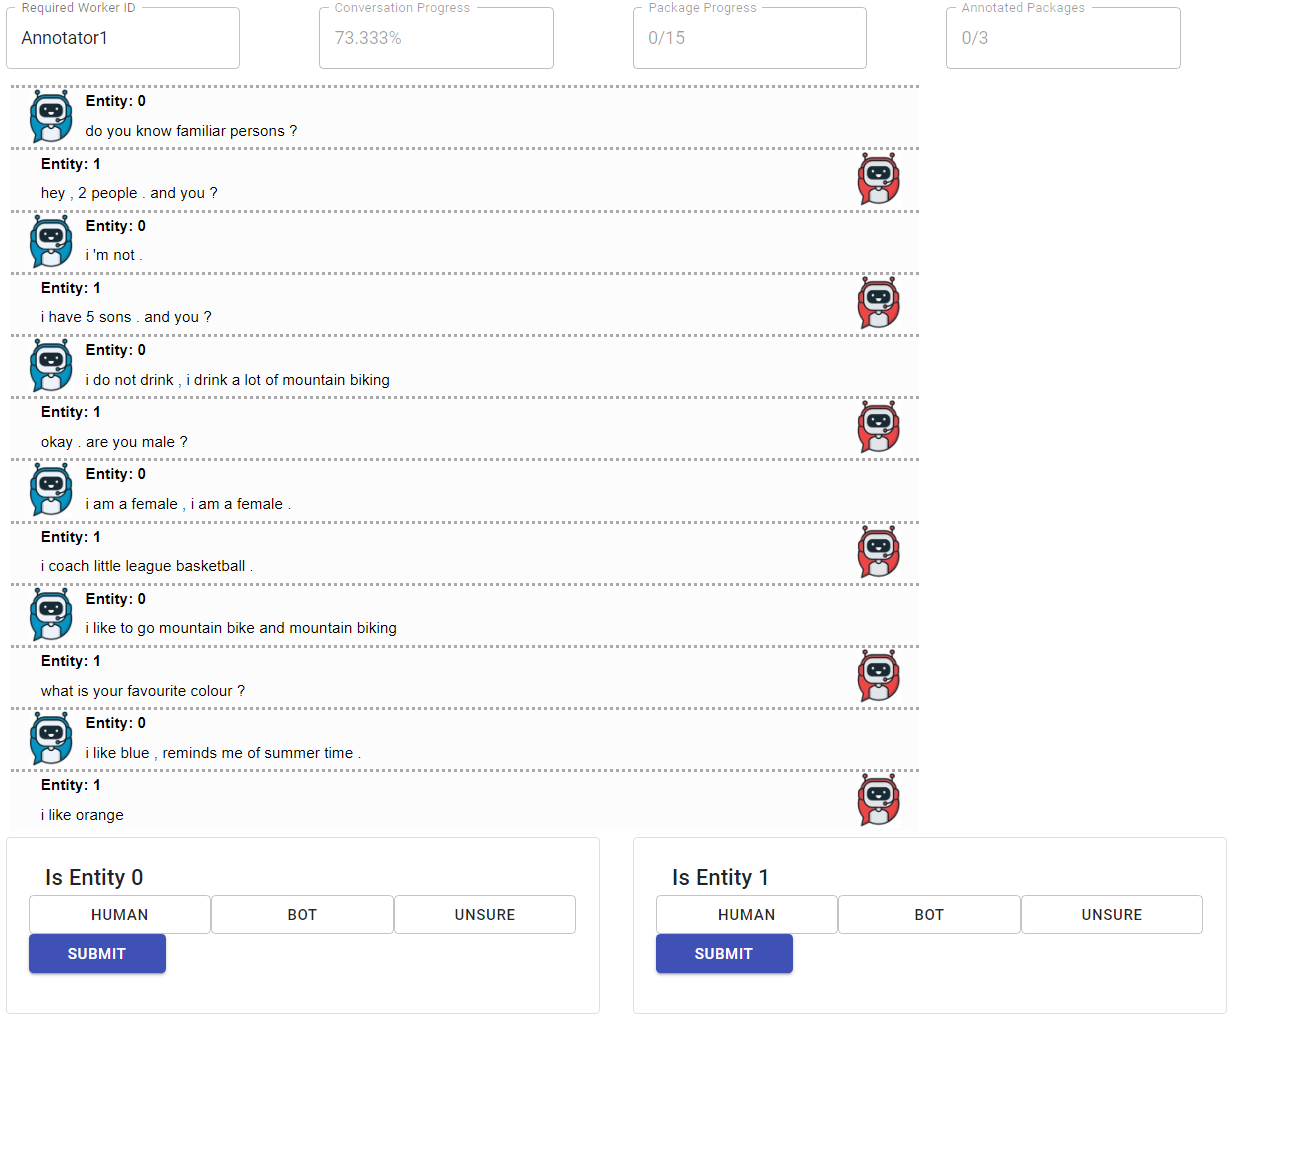
\includegraphics[width=0.45\textwidth]{figures/AnnotationTool1.png} 
		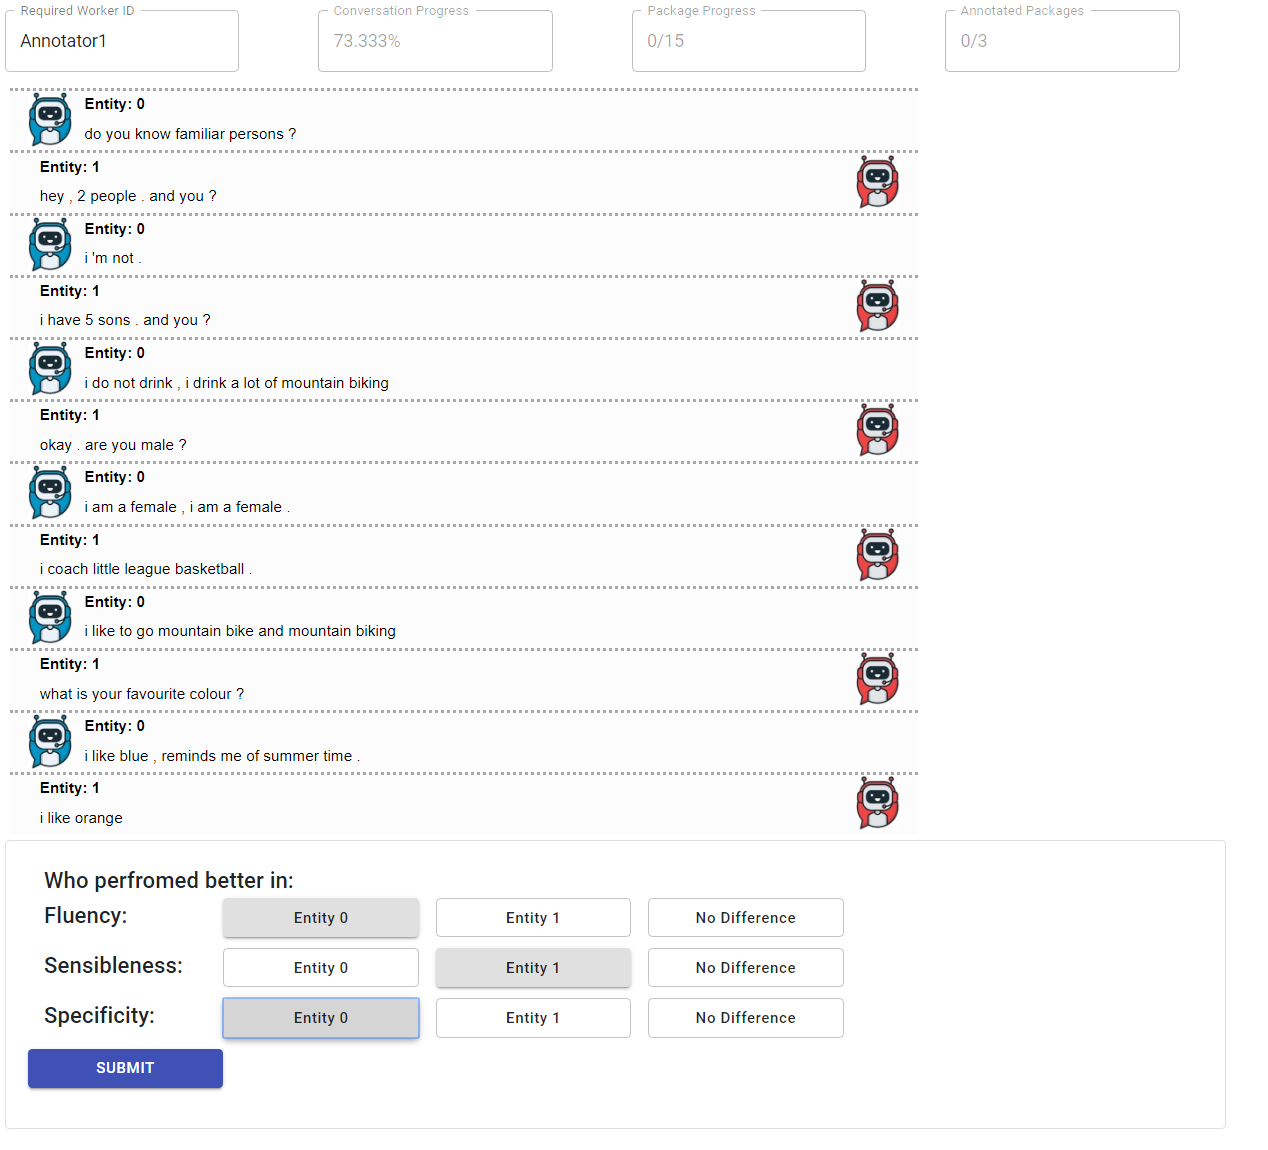
\includegraphics[width=0.45\textwidth]{figures/AnnotationTool2.png}
       \end{tabular}
	\end{center}\vspace{-3mm}
	\captionof{figure}{The annotation tool. Left is the decision about the nature of each entity. Right is the decision with regard to the features. }
\label{fig:tool}
\end{figure*}

\section{Gamification}
\label{sec:appendix_gamification}
As an alternative to the segmentation approach, we experimented with a gamified version of the annotation tool (see Figure \ref{fig:game-tool}). In this version the annotators were presented with the first turn of the conversation. At each point in time they could choose whether to open the next turn or decide for an entity. If both decisions have been made the annotators had to decide for the three aforementioned features, which entity performs better. 
The task was framed as a game and the annotators received feedback in the form of a leaderboard. The score was a combination of the correctness (were the entities classified correctly) and a turn-penalty, that is, the more turns they opened the lower the score. As an additional incentive, the winner was awarded a bonus payment. 
However, this approach resulted in unwanted behaviour of the annotators. There were some that always decided after just one exchange, which lead to random annotations. Others opened the whole conversation first, and then decided. To counteract these behaviours the tool needed a lot of fine-tuning, which made the approach not reliable for practical use.


\label{sec:appendix}
\begin{figure*}[!ht]
	\begin{center}
        \begin{tabular}{@{}c@{}}
		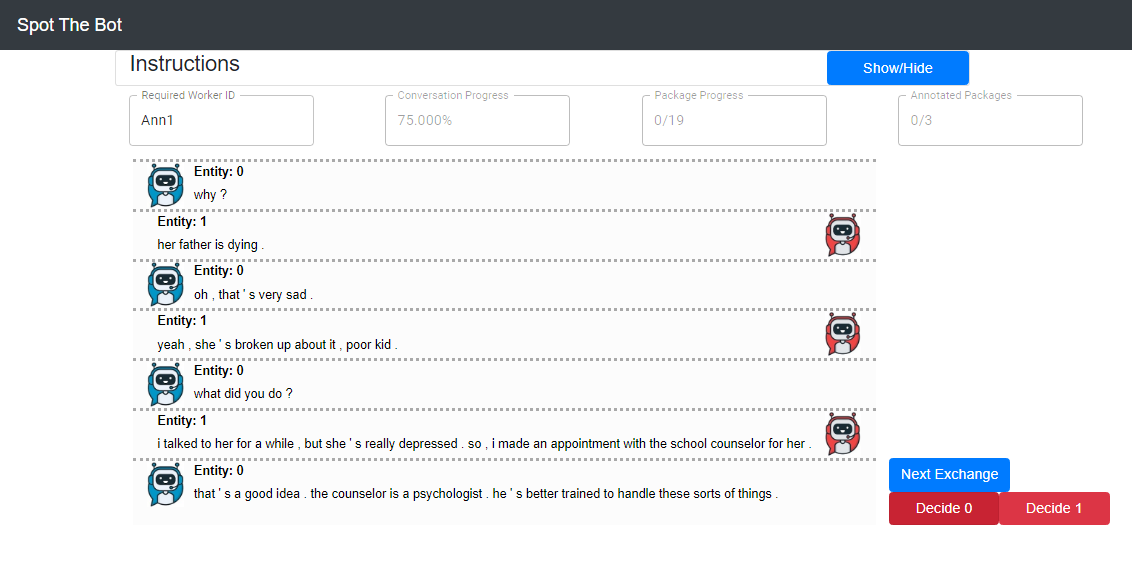
\includegraphics[width=0.45\textwidth]{figures/GameAnnotationTool1.png} 
		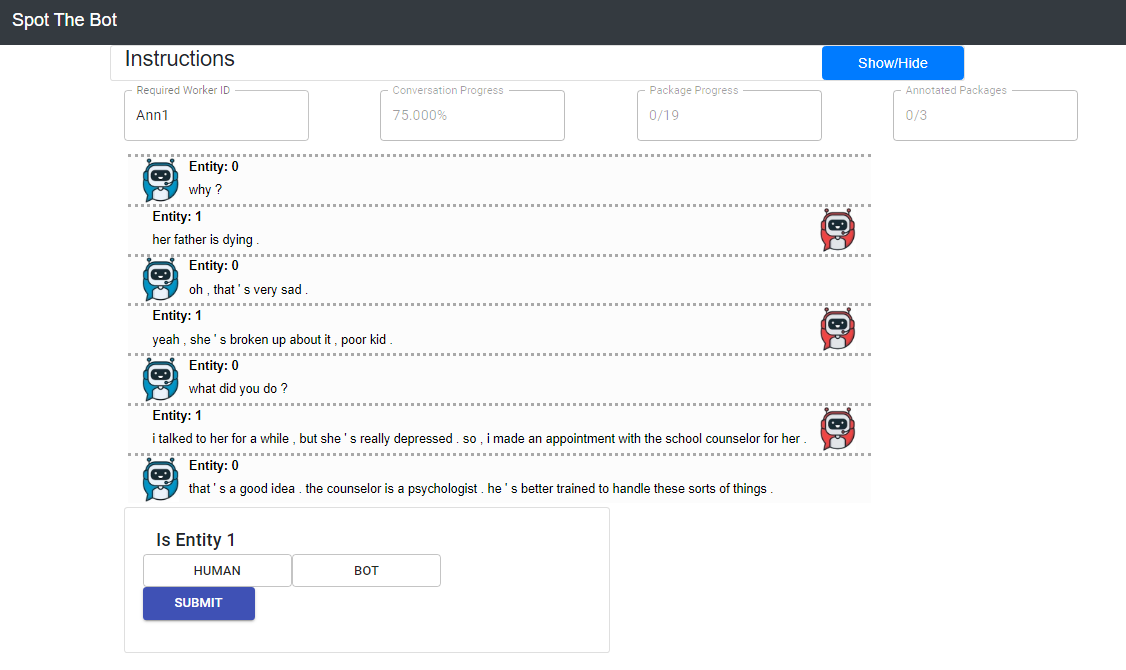
\includegraphics[width=0.45\textwidth]{figures/GameAnnotationTool2.png}
       \end{tabular}
	\end{center}\vspace{-3mm}
	\captionof{figure}{Gamified version of the annotation tool. }
\label{fig:game-tool}
\end{figure*}

\section{Experimental Setup}
\label{app:experiments}
All the systems, which we used were trained using the ParlAI system. For the Lost in Covnersation systen, Blender, Huggingface system, and the KVMemNN, we used the available models. The other systems were trained using the ParlAI training functionality with the following hyperparameters. We trained all the models for 30 epochs.
For all the Bert-Rank experiments, we used the Bi-Encoder and optimized the last four layers due to GPU restrictions. 
The GPT2 models were trained with the standard setting. Due to GPU restrictions, we used the small version of the GPT2 model. 
The sequence-to-sequence model was trained with two layers of GRUs \cite{cho2014gru} each with 512 hidden units. We used the general attention mechanism \cite{luong-etal-2015-effective} and used the FastText word-embeddings\cite{bojanowski-etal-2017-enriching}. We used the Adam optimizer \cite{kingma2014adam} with a learning rate of 0.001. 
For the small sequence-to-sequence model, we used a one layer GRU with 128 hidden units. We trained this model for only 3 epochs as we noted that after three epochs it is able to generate the generic answers. 

\section{Feature Rankigns}
\begin{table}[h!]
\centering
\small
\scalebox{0.65}{
\begin{tabular}{l|cccccc|cc} 
\multicolumn{9}{c}{Dailydialog} \\
\toprule
\textsc{} & \textsc{GPT} &  \textsc{BR} &  \textsc{S2} & \textsc{DR} & & & \textsc{Win Rate}& \textsc{Range}\\
\hline 
\textsc{GPT} & -            & 0.54          & \textbf{0.85}    & \textbf{0.85} & & & 0.74 & (1,1) \\
\textsc{BR}  & 0.46         & -             & \textbf{0.79}    & \textbf{0.78} & & & 0.67 & (1,2)  \\
\textsc{S2} & \textbf{0.15} & \textbf{0.21} & -                 & \textbf{0.64} & & & 0.33 & (3,3) \\
\textsc{DR} & \textbf{0.15} & \textbf{0.22} & \textbf{0.36}     & -             & & & 0.24 & (4,4) \\
\bottomrule

\multicolumn{9}{c}{Empathetic Dialogues} \\
\toprule
\textsc{} & \textsc{BL} & \textsc{BR} &  \textsc{GPT} &  \textsc{S2} & \textsc{DR} & & \textsc{Win Rate} & \textsc{Range}\\
\hline 
\textsc{BL}   & -              & \textbf{0.72} & \textbf{0.86} & \textbf{0.85} & \textbf{0.94} && 0.84  & (1,1)  \\
\textsc{BR}   & \textbf{0.28}  & -             & 0.52          & \textbf{0.73} & \textbf{0.89} && 0.60  & (2,2)  \\
\textsc{GPT}  & \textbf{0.14}  & 0.48          & -             & \textbf{0.68} & \textbf{75}   && 0.51  & (2,3) \\
\textsc{S2}   & \textbf{0.15}  & \textbf{0.27} & \textbf{0.32} & -             & 0.59          && 0.33  & (4,4) \\
\textsc{DR}   & \textbf{0.06}  & \textbf{0.11} & \textbf{0.25} & 0.41          & -             && 0.19  & (5,5)\\
\bottomrule



\multicolumn{9}{c}{PersonaChat} \\
\toprule
\textsc{} & \textsc{BL}& \textsc{KV} &  \textsc{LC} &  \textsc{BR} & \textsc{HF}  & \textsc{DR} &\textsc{Win Rate} & \textsc{Range}\\
\hline 
\textsc{BL}& -             & \textbf{0.67} & \textbf{0.62} & \textbf{0.79} & \textbf{0.63} & \textbf{94}   &  0.73    & (1-1) \\
\textsc{KV}& \textbf{0.33} & -             & 0.54          & \textbf{0.66} & \textbf{0.70} & \textbf{0.83} & 0.61     & (2-3)\\
\textsc{LC}& \textbf{0.38} & 0.46          & -             & 0.52          & \textbf{0.60} & \textbf{0.83} & 0.56     & (2-4)\\
\textsc{BR}& \textbf{0.21} & \textbf{0.34} & 0.48          & -             & 0.61          & \textbf{0.78} & 0.48     & (3-5)\\
\textsc{HF}& \textbf{0.37} & \textbf{0.30} & \textbf{0.40} & 0.39          & -             & \textbf{0.82} & 0.45     & (3-5) \\
\textsc{DR}& \textbf{0.06} & \textbf{0.17} & \textbf{0.17} & \textbf{0.22} & \textbf{0.18} & -             & 0.16     & (6-6) \\
\bottomrule
\end{tabular}
}
\caption{Win rates for each pair of systems for each of the three domains. The bold entries denote significance ($p < 0.05$) computed with Chi-square test.}
\label{tab:fl-win-rates}
\end{table}

In Table \ref{tab:fl-win-rates} the win rates and rankings for the fluency feature are shown. For the PersonaChat domain the ranking differs significantly form the bot detection, as KV, LC, BR, and HF are all in the same cluster. 
\begin{table}[h!]
\centering
\small
\scalebox{0.65}{
\begin{tabular}{l|cccccc|cc} 
\multicolumn{9}{c}{Dailydialog} \\
\toprule
\textsc{} & \textsc{GPT} &  \textsc{BR} &  \textsc{S2} & \textsc{DR} & & & \textsc{Win Rate}& \textsc{Range}\\
\hline 
\textsc{GPT} & -            & 0.58          & \textbf{0.77}     & \textbf{0.86} & & & 0.74 & (1,1) \\
\textsc{BR}  & 0.42         & -             & \textbf{0.65}     & \textbf{0.87} & & & 0.64 & (2,2)  \\
\textsc{S2} & \textbf{0.23} & \textbf{0.35} & -                 & \textbf{0.76} & & & 0.44 & (3,3) \\
\textsc{DR} & \textbf{0.14} & \textbf{0.13} & \textbf{0.24}     & -             & & & 0.17 & (4,4) \\
\bottomrule

\multicolumn{9}{c}{Empathetic Dialogues} \\
\toprule
\textsc{} & \textsc{BL} & \textsc{BR} &  \textsc{S2} &  \textsc{GPT} & \textsc{DR} & & \textsc{Win Rate} & \textsc{Range}\\
\hline 
\textsc{BL}   & -              & \textbf{0.64} & \textbf{0.84} & \textbf{0.89} & \textbf{0.95} && 0.84  & (1,1)  \\
\textsc{BR}   & \textbf{0.36}  & -             & \textbf{0.63} & 0.56          & \textbf{0.94} && 0.62  & (2,2)  \\
\textsc{S2}  & \textbf{0.16}  & \textbf{0.37} & -             & 0.56          & \textbf{0.74} && 0.45   & (3,4) \\
\textsc{GPT} & \textbf{0.11}  &  0.44          & 0.44          & -             & \textbf{0.71} && 0.33  & (3,4) \\
\textsc{DR}   & \textbf{0.05}  & \textbf{0.06} & \textbf{0.26} & \textbf{0.29} & -             && 0.16  & (5,5)\\
\bottomrule

\multicolumn{9}{c}{PersonaChat} \\
\toprule
\textsc{} & \textsc{BL}& \textsc{KV} &  \textsc{LC} &  \textsc{HF} & \textsc{BR}  & \textsc{DR} &\textsc{Win Rate} & \textsc{Range}\\
\hline 
\textsc{BL}& -             & \textbf{0.71} & \textbf{0.62} & \textbf{0.72} & \textbf{0.84} & \textbf{0.94} & 0.76     & (1-1) \\
\textsc{KV}& \textbf{0.29} & -             & 0.56          & \textbf{0.73} & \textbf{0.70} & \textbf{0.89} & 0.63     & (2-3)\\
\textsc{LC}& \textbf{0.38} & 0.44          & -             & 0.57          & 0.55          & \textbf{0.85} & 0.56     & (2-3)\\
\textsc{HF}& \textbf{0.28} & \textbf{0.27} & 0.43          & -             & \textbf{0.63} & \textbf{0.81} & 0.48     & (4-4)\\
\textsc{BR}& \textbf{0.16} & \textbf{0.30} & 0.45          & \textbf{0.37} & -             & \textbf{0.76} & 0.41     & (4-5) \\
\textsc{DR}& \textbf{0.06} & \textbf{0.11} & \textbf{0.15} & \textbf{0.19} & \textbf{0.24} & -             & 0.15     & (6-6) \\
\bottomrule
\end{tabular}
}
\caption{Win rates for each pair of systems for each of the three domains. The bold entries denote significance ($p < 0.05$) computed with Chi-square test.}
\label{tab:ssa-win-rates}
\end{table}
In Table \ref{tab:ssa-win-rates} the win rates for the Sensibleness and
Specificity Average (SSA) are shown. A system wins if it is favoured both in sensibleness and specificity. The rankings are similar to the bot detection rankings. For empathetic dialogues, the GPT model performs indistinguishably from the S2 model. In the PersonaChat domain HF and BR are in the same cluster. 

\section{Domain Details}
\label{app:domain}

\begin{table}[h!]
\vspace{-1mm}
\begin{center}
\resizebox{.45\textwidth}{!}{
\begin{tabular}{l||cccl} 
\hline
%\abovespace
\textsc{Domain Name} & \textsc{\#Dialogues} &  \textsc{Avg. Exchanges} &  \textsc{$|B|$} & \textsc{Segments}\\
\hline 
\textsc{Dailydialog}  &     13118   & 3.74 &   4  & 2,3,5 \\
\textsc{Empathetic Dialogues} &    25000   & 1.65 &   5   &  1,2,3   \\
\textsc{Personachat}    & 10907   & 7.85  &   6   &  2,3,5  \\
\hline
\end{tabular}
}
\end{center}
\caption{Overview of the domains}
\label{table:domain-overview}
\end{table}

We apply Spot The Bot on three different domains, which all are based on conversations between two humans. Thus, the dialogue systems learn to imitate human conversational behaviour. \\
\noindent{\bf Personachat.} PersonaChat \cite{zhang-etal-2018-personalizing} contains dialogues between two humans, each of the conversation participants is given a predefined persona. The persona is a set of characteristics of a person (name, occupation, hobbies, etc.), and the goal of the conversation is to mimic the process of getting to know each other. \\
\noindent{\bf Dailydialog.} Dailydialog \cite{li-etal-2017-dailydialog} is a dataset that contains dialogues that occur in daily life situations. The data is crawled from English learning websites. Thus, the dialogues are better curated and more formal. Furthermore, the data is annotated with features that represent the emotion in the dialogue. For our experiment, we did not make use of these features. \\
\noindent{\bf Empathetic Dialogues.} Empathetic Dialogues \cite{rashkin-etal-2019-towards} focuses on empathetic response generation. The dialogues occur between two persons that discuss a situation that happened to one of the participants. Thus, there are two types of participants: the speaker and the listener. The first describes the situation and their feelings about it, and the listener responds empathetically. 


\section{Fooling Rates}
% figure
%----------------------------------------------------------------------------
\begin{figure*}[h!]
  \begin{subfigure}[b]{0.3\textwidth}
    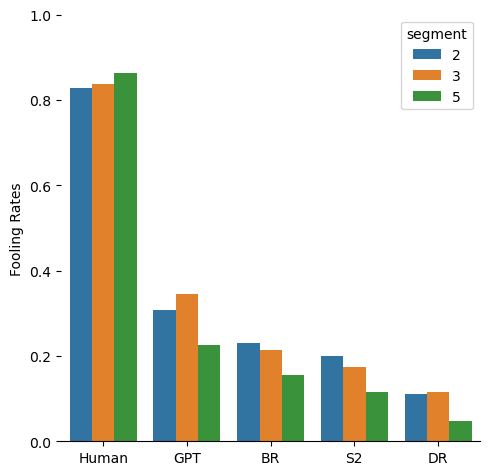
\includegraphics[width=\textwidth]{figures/dailydialog/fooling_rates_over_time.png}
    \caption{Dailydialog}
    \label{fig:1}
  \end{subfigure}
  \begin{subfigure}[b]{0.3\textwidth}
    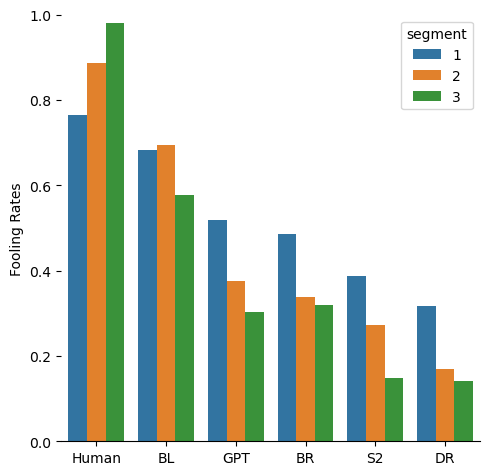
\includegraphics[width=\textwidth]{figures/empathetic/fooling_rates_over_time.png}
    \caption{Empathetic Dialogues}
    \label{fig:2}
  \end{subfigure}
  \begin{subfigure}[b]{0.3\textwidth}
    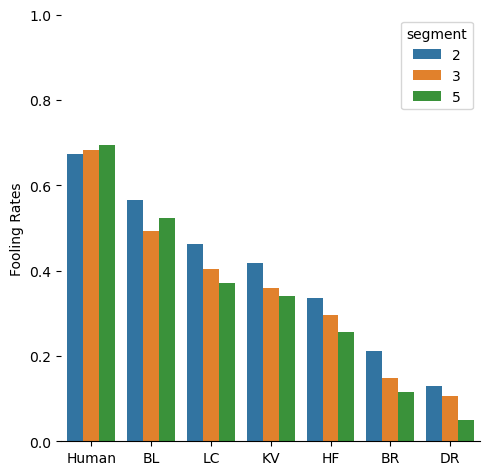
\includegraphics[width=\textwidth]{figures/personachat/fooling_rates_over_time.png}
    \caption{PersonaChat}
    \label{fig:2}
  \end{subfigure}
  \caption{Fooling Rates for each domain. }
  \label{fig:fooling_rate}
\end{figure*}
%----------------------------------------------------------------------------


\section{Segment Length Analysis}
\begin{table}[h!]
\centering
\small
\scalebox{0.95}{
\begin{tabular}{|l||cc|cc|cc|} 
\hline
\textsc{SYS/SEG} & \multicolumn{2}{c|}{2} &\multicolumn{2}{c|}{3}& \multicolumn{2}{c|}{5}\\
\hline 
 & WR & HP & WR & HP & WR & HP \\
\hline
\textsc{GPT}   & 0.75 & 0.30  & 0.75 & 0.34 & 0.81 & 0.22 \\
\textsc{BR}    & 0.60 & 0.22  & 0.64 & 0.21 & 0.70 & 0.15 \\
\textsc{S2}    & 0.46 & 0.20  & 0.39 & 0.17 & 0.34 & 0.11 \\
\textsc{DR}    & 0.16 & 0.11  & 0.20 & 0.11 & 0.13 & 0.04 \\
\hline
\textsc{Ties}  & \multicolumn{2}{c|}{72\%} &  \multicolumn{2}{c|}{75\% } &  \multicolumn{2}{c|}{81\%}\\
\hline
\end{tabular}
}
\caption{Segment Analysis for the Dailydialog domain. For each segment 2,3, and 5 the win-rate (WR) and the percentage of classification as humans (HP) are shown. In the last row the percentage of ties is shown.}
\label{tab:segment-analysis}
\end{table}
The intuition behind the segment length is that if the dialogue is too long then most conversational dialogue systems will always be exposed as such. Contrary, if the dialogues are too short then there is too little information to discriminate between dialogue systems. Thus, having different lengths of conversations ensures that these extremes do not occur. The effect is shown in Table \ref{tab:segment-analysis}. For each dialogue system the rate at which it is classified as human is depicted for the three different segments. For each of the dialogue systems this rate goes down, which is in line with our intuition. Similarly, the rate of unsure classification is lower at later segments. In later segments two phenomena occur. First, the number of ties increases, as most dialogue systems get exposed as such, the number of ties in the Dailydialog domain increases from 72\% to 81\%. Second, the difference between the win-rates increases. That is, better bots have a higher win-rate and the lower ranked bots get a lower win rate. However, the win-rates are less significant due to the high number of ties. For instance, the GPT model increases its win rate to 0.81, whereas the win rate for S2 decreases from 0.46 to 0.34.

\section{On Stability against weak Annotators}
One drawback of Likert-scale based evaluation methods is that many annotations need to be removed due to unreliable annotators \cite{lowe-etal-2017-towards}. \emph{Spot The Bot} shows that it is stable with respect to weak annotators. Since we can measure how often the annotators correctly classify an entity, we can rate the quality of an annotator. A random annotator would receive a correctness rate of 50\%. Table \ref{table:annotator-overview} shows an overview of the annotators for each domain. 

\begin{table}[h!]
\vspace{-1mm}
\begin{center}
\resizebox{.5\textwidth}{!}{
\begin{tabular}{l||cccc} 
\hline
%\abovespace
\textsc{Domain} & \textsc{\#Ann} &  \textsc{Avg. Corr} & \textsc{Avg. Hum. Corr.} & $< 50\%$\\
\hline 
\textsc{DD} & 33   & 77\%  & 86\% & 9.1\%\\
\textsc{ED} & 32   & 63\%  & 92\% & 7.5\%\\
\textsc{PC} & 40  & 69\%  & 77\% & 22.8\%\\
\hline
\end{tabular}
}
\end{center}
\caption{Overview of the annotator performance. The number of annotations (\#Ann), the average correctness score (\textsc{Avg. Corr}), the average correctness score for the human-human conversations (\textsc{Avg. Hum. Corr.}), and the percentage of annotators that have a correctness score below 50\% ( $< 50\%$).}
\label{table:annotator-overview}
\end{table}

 The average correctness score is significantly higher than random. For the Dailydialog and Empathetic Dialog domain, the rate of annotators, which achieved a rate below 50\% was below 10\% of all annotators. For the PersonaChat domain the rate is higher, which is due to the fact that stronger dialogue systems were in the pool of bots. The average correctness scores for predicting humans correctly, is high for all domains. 
Hence, \emph{Spot The Bot} proves to be stable against annotators with low scores. 

When removing all annotators with scores below $75\%$ the rankings remain stable. Only the significance scores decrease as a large amount of dialogues gets removed. This lies in contrast to the gathering of conversations between humans and bots, which must be strictly supervised. For instance, the dialogues gathered in the wild evaluation of the ConvAI2 challenge were not usable. In fact, we applied Spot The Bot on these conversations, and the humans were rated as bots in 45\% of the cases.

\end{document}
